%\documentclass[a4paper,fleqn,longmktitle]{cas-dc}
\documentclass[a4paper,fleqn]{cas-dc}

%\usepackage[authoryear,longnamesfirst]{natbib}
%\usepackage[authoryear]{natbib}
\usepackage[numbers]{natbib}
\usepackage{listings}
\usepackage{color}
\usepackage{tabularx}
\usepackage{wrapfig}
%\renewcommand{\arraystretch}{2}
\usepackage{float}

\begin{document}

    \shorttitle{Harpe: Using Adversarial Machine Learning to dodge Intrusion Detection Systems in Software-Defined
    Perimeters}
    \shortauthors{Antonio Paya, Sergio Arroni, Vicente García and Alberto Gómez}

% ============================== TITLE
    \title [mode = title]{Harpe: Using Adversarial Machine Learning to dodge Intrusion Detection Systems in
    Software-Defined Perimeters}


% ============================== AUTHORS
    \author[uniovi]{Antonio Paya}[orcid=0000-0003-3733-3805]\ead{antoniopaya@outlook.com}\cormark[1]

    \author[uniovi]{Sergio Arroni}[orcid=0000-0002-4907-8576]\ead{sergioadgi38@gmail.com}

    \author[uniovi]{Vicente García-Díaz}[orcid=0000-0003-2037-8548]\ead{garciavicente@uniovi.es}

    \author[epi]{Alberto Gómez}[orcid=0000-0003-2037-8548]\ead{albertogomez@uniovi.es}

    \address[uniovi]{Department of Computer Science,
        University of Oviedo, Science Faculty, Oviedo, Spain}
    \address[epi]{Department of Business Administration, University of Oviedo, Gijón, Spain}

    \cortext[cor1]{Corresponding author}
% ============================== ABSTRACT
    \begin{abstract}
        With the increasing reliance on \textit{Software-Defined Perimeters} (\textit{SDPs}) for network security, it
        is important to understand the limitations and vulnerabilities of this architecture.
        This paper proposes a framework, \textit{Harpe}, that generates attacks on \textit{SDP}-based networks to
        demonstrate the potential weaknesses of this architecture.
        \textit{Harpe} generates malicious network traffic that mimics normal traffic to evade the
        \textit{Intrusion Detection System} (\textit{IDS}) component of \textit{SDPs}.
        Utilizing \textit{Adversarial Machine Learning} techniques, it learns how the \textit{IDS} operates and finds
        ways to evade detection.
        The effectiveness of the proposed framework is tested in two different environments, a traditional network
        architecture and an \textit{SDP}-based network.
        The results show that \textit{Harpe} is capable of significantly reducing the detection capabilities of the
        \textit{IDS} in both environments, highlighting the need for further research and improvement of \textit{SDP}
        security mechanisms.
    \end{abstract}

% ============================== KEYWORDS
    \begin{keywords}
        Adversarial Machine Learning \sep Software-Defined Perimeters \sep Intrusion Detection Systems \sep Artificial Intelligence
        \sep Cybersecurity \sep W-GAN 
    \end{keywords}


    \maketitle

%% main text
%% ============================================================ I. Introduction


    \section{Introduction}\label{sec:introduction}
    %TODO: Introduction
As computer networks continue to grow in size and complexity, the need for effective security measures becomes
increasingly critical.
Intrusion Detection Systems (IDS) have been developed to address this challenge, providing a means of monitoring
network traffic and identifying potential security threats.
These systems can analyze network traffic and identify potential security threats such as malware, network intrusions,
and denial of service attacks.
However, the increasing complexity and diversity of network traffic have made it difficult to accurately classify
network traffic using traditional rule-based IDS systems~\cite{thakkar2020review}.

To overcome these limitations, Machine Learning (ML) techniques have been widely adopted in IDS for network traffic
classification.
These techniques leverage the power of statistical models and algorithms to automatically learn and detect anomalous
network traffic patterns, which are indicative of security threats.

ML-based IDS systems offer several advantages over traditional rule-based systems, including higher accuracy, better
scalability, and more robustness to evolving network threats~\cite{abdallah2022intrusion, maseer2021benchmarking}.
However, they also pose new challenges, particularly in terms of security.
One of the main challenges is the susceptibility of ML models to Adversarial Machine Learning (AML)
attacks~\cite{huang2011adversarial}.

AML attacks are a type of cyber-attack that aims to manipulate ML models by feeding them carefully crafted input data,
called adversarial examples.
These examples are designed to cause misclassification or incorrect predictions, which can be exploited by attackers to
bypass the security measures of IDS systems~\cite{zhao2021attackgan, lin2022idsgan, liu2022vulnergan}.

Attackers create adversarial examples by utilizing information obtained from the targeted IDS, including its responses
to specific inputs.
This information is used to train a model capable of generating adversarial traffic that remains undetectable by the
IDS classifier.

As ML-based IDS systems become more prevalent, the threat of Adversarial Machine Learning (AML) attacks becomes more
significant~\cite{duy2021digfupas}.
Therefore, it is crucial to develop effective defense mechanisms to mitigate the impact of these attacks and ensure the
reliability and robustness of IDS systems.

In this paper, we propose a new robust defense system against Adversarial Machine Learning attacks on Intrusion
Detection Systems called \textit{Apollon}.
\textit{Apollon} serves to safeguard IDS from attackers by obstructing their ability to generate adversarial traffic through
learning from the behavior of the IDS.

\textit{Apollon} utilizes a diverse range of classifiers to detect intrusions and employs a \textit{Multi-Armed Bandits (MAB)}
model to select the best-suited classifier or a combination of classifiers in real-time for each input, enabling it to achieve
this objective without compromising its performance on normal inputs.

In this way, \textit{Apollon} can prevent attackers from learning the behavior of the IDS in realistic training times, adding a
layer of semi-randomness to the IDS behavior that makes it more difficult for attackers to detect the IDS behavior and
generate adversarial traffic.

The structure of the paper is as follows.
Section ~\ref{sec:background} provides an overview of the main concepts and techniques used in this paper.
Section ~\ref{sec:related-work} discusses the related work in the field of AML attacks and IDS classifiers.
Section ~\ref{sec:proposal} presents the proposed defense system, \textit{Apollon}.
Section ~\ref{sec:evaluation} presents the experimental evaluation of \textit{Apollon}.
Finally, Section ~\ref{sec:conclusions-and-future-work} concludes the paper and discusses future work.

%% ============================================================ I. Background


    \section{Background}\label{sec:background}
    In this section, we will provide an overview of the concept of \textit{Software-Defined Perimeters (SDP)} and their
role in network security.
Next, we will discuss the concept of \textit{Intrusion Detection Systems (IDSs)}, the available datasets, and their role
in the context of \textit{SDPs}.
Finally, we will also discuss the basics of \textit{Adversarial Machine Learning (AML)} and its potential for
exploitation in cyberattacks.
This information will provide the necessary context for the subsequent sections of this paper.

\subsection{Software-Defined Perimeters}\label{subsec:software-defined-perimeters}

The \textit{Software-Defined Perimeter (SDP)} is a security framework developed by the Cloud Security Alliance (CSA) to
dynamically protect networks~\cite{Koilpillai2020, Kumar2019}.
The \textit{Software-Defined Perimeter} framework was adapted from the \textit{Global Information Grid (GIG) Black Core}
initiative proposed by the USA Department of Defense (DoD)~\cite{Enterprise2007}.
The CSA modified the generalized DoD workflow for commercial use and aligned it with National Institute of Standards
and Technology (NIST) security controls.
The \textit{SDP} follows a strategy based on the \textit{Zero Trust} security model, where the identity of the device or
application that will initiate the communication is verified and authenticated before granting access to the
infrastructure~\cite{rose2020zero}.

In this model, there is a clear separation between its two main components (\textit{PDP} and \textit{PEP}),
which operate in the control plane and data plane respectively.
The \textit{Policy Decision Point (PDP)} includes trust and policy engines where authorization and access
decisions are made based on the information provided by the \textit{Policy Enforcement Point (PEP)}.

The architecture of SDP frameworks consists of three main components (see Figure~\ref{fig:sdp}).

\begin{figure*}
    \centering
    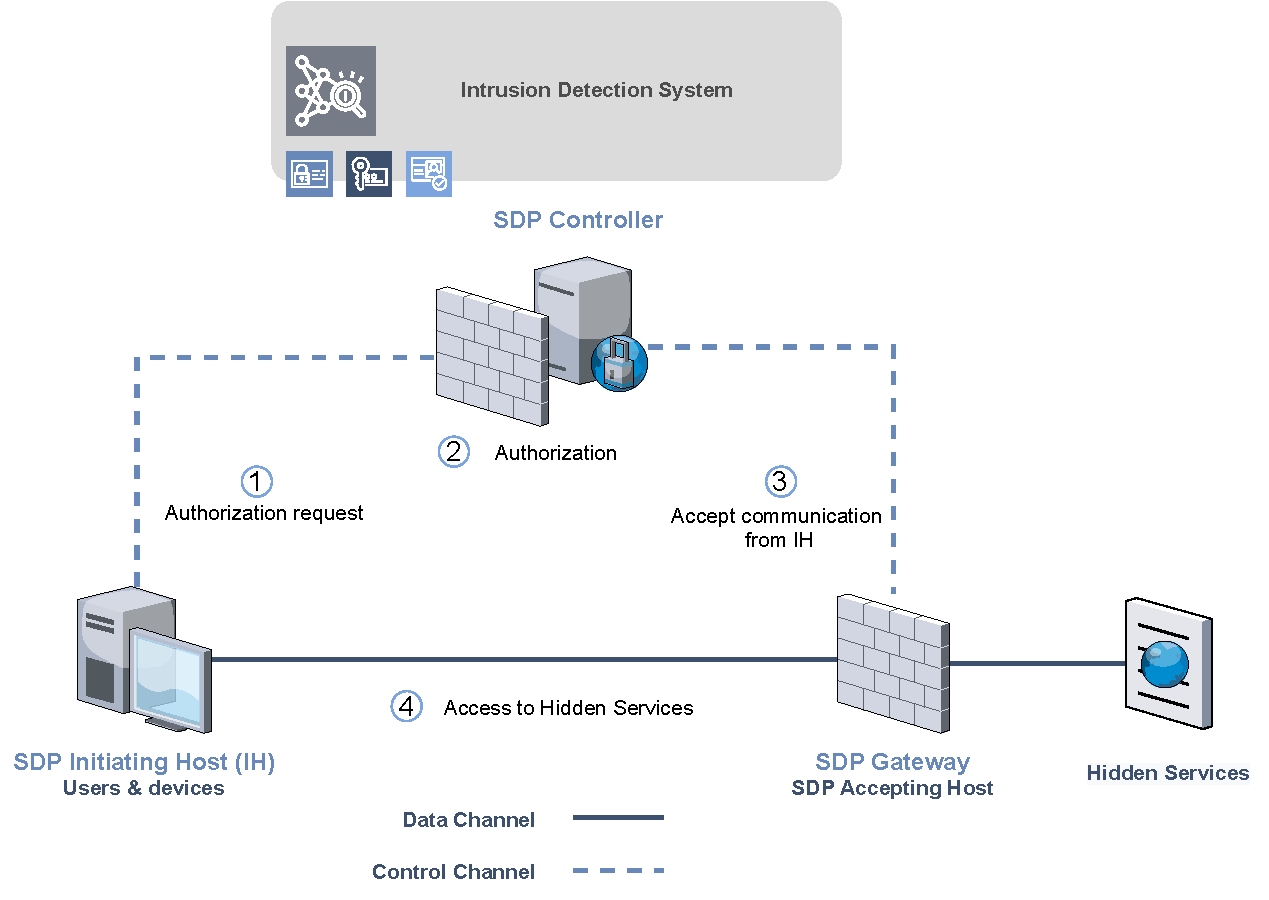
\includegraphics[width=.7\textwidth]{Figures/SDP}
    \caption{\label{fig:sdp} \textit{Software-Defined Perimeter} architecture~\cite{CSAZeroTrust2020}}
\end{figure*}


\subsubsection{SDP Controller}
The \textit{SDP Controller} is the central component of the \textit{SDP} framework and plays a crucial role in the
exchange of control messages.
It acts as a trusted agent between the \textit{SDP Initiating Host} and the backend security controls.
The \textit{SDP Controller} includes tasks for device identification and authentication, as well as determining which
programs or services are authorized for each device ~\cite{Koilpillai2020, Kumar2019}.
These tasks are crucial for the proper functioning of \textit{Intrusion Detection Systems (IDS)}, which are used to
identify and alert on unauthorized access or malicious activity within the network.

\subsubsection{SDP Initiating Host}
The \textit{SDP Initiating Host} is the device that initiates the connection to the backend security controls.
This device is responsible for sending the control messages to the \textit{SDP Controller} and for receiving the
authorization response from the \textit{SDP Controller} ~\cite{Koilpillai2020, Kumar2019}.
Once the authentication is completed, a mutual \textit{TLS tunnel} is created that connects the client (IH) to the
service or application for which it has authentication.

\subsubsection{SDP Accepting Host or Gateway}
\textit{Accepting Hosts} are the devices that are instructed to accept certain authorized services or applications.
The \textit{SDP Accepting Host} is protected by a firewall that allows only the authorized services or applications to
communicate with the \textit{SDP Initiating Host} ~\cite{Koilpillai2020, Kumar2019}.


\subsection{Intrusion Detection Systems}\label{subsec:intrusion-detection-systems}
\textit{Intrusion Detection Systems (IDS)} are security technologies designed to detect and alert on unauthorized
access or malicious activity within a network.
They are an important tool in protecting against cyber threats, such as malware, viruses, and hacking attempts.
\textit{IDSs} can operate in real-time, analyzing network traffic as it occurs, or they can be configured to analyze
logs or other stored data.
They use a variety of techniques to detect intrusions, such as analyzing network traffic patterns, examining system
logs, and looking for known malicious activity indicators.
\textit{IDSs} play a critical role in maintaining the security and integrity of a network, and are commonly used in
conjunction with other security measures such as firewalls and antivirus software.

\textit{Machine Learning (ML)} techniques have increasingly been used in \textit{IDSs} in recent
years~\cite{abdallah2022intrusion, thakkar2020review, maseer2021benchmarking} due to their ability to analyze large
amounts of data and identify complex patterns that might not be easily detected by traditional rule-based approaches.
\textit{ML-based IDSs} are capable of learning from past data and adapting to new patterns of behavior, which makes
them more effective at detecting new and evolving threats.
Additionally, \textit{ML} can be used to improve the accuracy and efficiency of \textit{IDSs} by reducing the number of
false positives and false negatives.

\subsection{Datasets overview}\label{subsec:datasets-overview}

\textit{Intrusion Detection Systems} datasets are an important resource for evaluating and benchmarking the performance
of \textit{IDSs}.
This datasets are typically collections of labeled examples of normal and abnormal network traffic, which are used to
train and test the accuracy and effectiveness of \textit{IDSs}.
There are several datasets available, each with its own characteristics and strengths.
In this part, we will review some of the most popular datasets and discuss their key features and uses.

\subsubsection{CIC-IDS2017}
The \textit{CIC-IDS2017} dataset~\cite{CICIDS2017} was created in a simulated enterprise network environment and captures
network traffic data over a five-day period.
The data was collected to mimic the behavior of 25 users and contains approximately 80 significant
attributes~\cite{RING2019147}.
It is currently one of the most widely used \textit{IDS} datasets in modern literature and contains a high ratio of
benign to malicious examples (83\% vs 17\%).
It can be used individually or in conjunction with other datasets, as it accurately reflects the normal distribution of
benign and malicious traffic in a network \cite{Shroff2022}.

\subsubsection{CSE-CIC-IDS2018}
The \textit{CSE-CIC-IDS2018} dataset~\cite{CSE-CIC-IDS2018}, created by the Canadian Institute for Cybersecurity (CIC),
was collected in a simulated enterprise network environment using AWS resources in 2018.
It contains data on seven different attack types and has approximately 79 significant features .
The dataset includes data from over 450 devices, including servers, computers, and other devices, and is notable for
its large size and high level of realism \cite{pujari2022comparative}.
It is similar to the \textit{CIC-IDS2017} dataset in that it includes packet analysis of network traffic with
bidirectional flow, but is larger and more comprehensive.
As a result, it is widely used in the literature for evaluating and benchmarking IDSs \cite{pujari2022comparative}.

\subsubsection{CIC-DDoS2019}
The \textit{CIC-DDoS2019} dataset~\cite{CICDDoS2019} was created to address the lack of representation of all subtypes
of DDoS attacks in existing datasets.
While the dataset includes simulated network traffic, efforts were made to create realistic benign data.
It includes 13 types of DDoS attacks and has more than 80 significant features.
However, the dataset is heavily imbalanced, with 50,006,249 records of DDoS attacks and only 56,863 records of benign
traffic, making it difficult to use for training a model on both types of data \cite{RING2019147}.
It is therefore recommended to use this dataset in conjunction with other datasets, such as \textit{CIC-IDS2017} or
\textit{CSE-CIC-IDS2018}, to train a more robust model \cite{Shroff2022}.

\subsubsection{ADFA IDS - UNSW-NB15}
The \textit{UNSW-NB15} dataset~\cite{UNSW-NB15} was developed at the University of New South Wales (UNSW) in Canberra
by the Cyber Range laboratory.
It is notable for its use of raw network packets that are a hybrid of real normal activities and synthetic contemporary
attack behaviors.
The dataset includes nine attack types and a total of 49 features, and is correctly labeled \cite{RING2019147}.
Unlike many other \textit{IDS} datasets, the \textit{UNSW-NB15} dataset is well-balanced, making it an excellent choice
for training models.

\subsubsection{Unused datasets}
There are many other \textit{IDS} datasets, such as \textit{Darpa 1998/99}~\cite{darpa1999},
\textit{KDD 99}~\cite{KDDCUP99} or \textit{NSL-KDD}~\cite{KDDCUP99}, which have not been used in this project.
The \textit{Darpa 1998/99} and \textit{KDD 99} datasets are no longer commonly used for evaluating and benchmarking
\textit{IDS} due to their outdated nature.
These datasets were created in the late 1990s and early 2000s, and do not accurately reflect the current landscape of
network threats and behaviors.
In particular, the \textit{KDD 99} dataset has been criticized for its high rate of false positives and its lack of
realism, which makes it less useful for testing the performance of modern \textit{IDS}~\cite{hugh2000, KDDFaults}.

On the other hand, datasets such as \textit{UNSW-NB15} and \textit{CIC-IDS2017} are more widely used due to their
larger size, greater realism, and more balanced distribution of benign and malicious examples .

\subsection{Adversarial Machine Learning}\label{subsec:adversarial-machine-learning}

\textit{Adversarial Machine Learning (AML)} refers to the use of \textit{Machine Learning} techniques to deceive or
mislead models.
According to the taxonomy of the attack and with Emiliano de Cristofaro \cite{de2020overview}, they can be classified into poisoning attacks, evasion attacks, inference
attacks, and extraction attacks.

\begin{itemize}
    \item \textbf{Poisoning attacks}: This attack involves modifying the training data in a way that causes the model to perform
    poorly on specific types of inputs.
    These attacks can be targeted at specific data points or can be more general, affecting the model's overall
    performance.
    Poisoning attacks can be difficult to detect, as the modified data can be indistinguishable from normal data.

    \item \textbf{Evasion attacks}: This attack involves generating inputs that are specifically designed to evade detection by the
    model.
    These inputs, known as adversarial examples, are modified versions of normal inputs that have been slightly
    perturbed in a way that is not easily noticeable to humans, but can cause the model to misclassify them.
    Evasion attacks can be conducted using a variety of techniques, such as gradient-based optimization or \textit{ML}.

    \item \textbf{Inference attacks}: This attack consists of inverting the sense of the information in a Machine Learning model. 
    The purpose is to get information from the model, which was not intended to be shared.
    There are three main sub-types of inference attack,
    \textit{Membership Inference Attack (MIA)} which is to discover whether or not a piece of data has been used in training,
    \textit{Property Inference Attack (PIA)} which attempts to infer model parameters and statistics,
    and Data Reconstruction which attempts to replicate the training samples.


    \item \textbf{Extraction attacks}: This attack is based on obtaining data from Machine Learning models.
    It uses a series of requests to the model, which allows it to intuit or predict the behavior of a model.
    These attacks can be easily detected as they need to send many suspicious requests.
    This type of attack it is intended to reveal the inner workings of the model,
    once enough knowledge is obtained, the model can be replicated or profit can be made from this information.  


\end{itemize}

In the context of \textit{IDSs}, \textit{AML} can be used to attack the \textit{IDS} by generating adversarial examples
that are designed to evade detection.
These attacks can be difficult to defend against~\cite{kariyappa2020defending}, as they rely on the ability to generate
inputs that are specifically designed to deceive the \textit{IDS}.
Some of the most common evasion attacks types used in \textit{IDS} are the \textit{Model extraction attacks} and the
\textit{Input reconstruction attacks}.
In this context, and depending on the level of knowledge of the attacker, adversarial attacks can be classified into
three types:

\begin{itemize}
    \item \textbf{White-box attacks}: In a white-box attack, the attacker has complete access to all information about
    the ML-based \textit{IDS}, including the training data and learning model architecture, decision and parameters
    (gradient, loss function, etc.).
    This gives the attacker a significant advantage, but fortunately, this type of attack is generally not practical
    in most real-world situations.

    \item \textbf{Black-box attacks}: In a black-box attack, the attacker has no knowledge of the \textit{IDS} model
    architecture, parameters, or training data.

    \item \textbf{Gray-box attacks}: Gray-box attacks involve an attacker who has some level of knowledge about the
    ML-based \textit{IDS} and may have limited access to the training data.
    In this scenario, the attacker does not have complete information about the system, but has enough information to
    attack it and cause it to fail.
    This type of attack is considered more realistic because it takes into account the fact that an attacker may
    have partial knowledge of the system they are targeting.
\end{itemize}

It is worth noting that in academic literature, the term ``black-box attacks'' is sometimes used to refer to
``gray-box attacks''.
In this article, we use the terms ``gray/black-box'' to refer specifically to the type of gray-box attacks
described above, to distinguish them from the more general use of the term ``black-box'' in the literature.

%% ============================================================ III. Related Work


    \section{Related Work}\label{sec:related-work}
    In this section, we will review the different \textit{IDS} classifiers and their scores for the selected datasets.
These classifiers will be utilized later to simulate the \textit{SDP IDS}.
Furthermore, we will detail the various types of \textit{AML} attacks that are employed in this context.

\subsection{Intrusion Detection Systems classifiers}\label{subsec:intrusion-detection-systems-classifiers}

As the number and sophistication of malware threats continue to grow, it is increasingly important to have effective
\textit{IDS} in place to protect network systems.
To ensure the effectiveness of \textit{IDS} systems, researchers conduct a range of studies and literature reviews to
identify and address potential vulnerabilities.
These studies are ongoing and are crucial in the ongoing development of \textit{IDS} systems to keep pace with the
evolving threat landscape.

Tables~\ref{tab:ids-classifiers-cic-ids2017},~\ref{tab:ids-classifiers-cse-cic-ids2018},
~\ref{tab:ids-classifiers-cic-ddos2019}, and~\ref{tab:ids-classifiers-unsw-nb15} show the \textit{IDS} classifiers and
their scores (accuracy, F1, and AUC) for the \textit{CIC-IDS2017}, \textit{CSE-CIC-IDS2018}, \textit{CIC-DDoS2019}, and
\textit{UNSW-NB15} datasets, respectively.
In these datasets and the most commonly used datasets (\textit{KDDD 99} and \textit{NSL-KDD}), the most commonly used
and best-performing classifiers are \textit{Random Forest}, \textit{Decision Trees}, and \textit{SVM}.
\textit{Random Forest}~\cite{zhang2008random}, in particular, has gained popularity due to its ability to handle large
datasets and its robust performance when dealing with noise and missing values in the data.
\textit{Decision Trees}~\cite{amor2004naive} are also popular due to their interpretability and simplicity, as they
allow for clear visualization of the decision-making process.
\textit{SVMs}~\cite{mohammadi2021} are favored for their ability to handle high-dimensional data and their versatility
in dealing with different types of classification tasks.
Overall, these classifiers have demonstrated strong performance and are frequently used in the field of \textit{IDS}.

\begin{table}
    \resizebox{\columnwidth}{!}{%
        \begin{tabular}{|r|rrr|l|}
            \hline
            \textbf{Classifier} & \textbf{Accuracy} & \textbf{F1 score} & \textbf{AUC} & \textbf{Ref}                                                                                     \\ \hline
            IGAN-IDS            & 99.79             & 99.79             & 99.98        & ~\cite{huang2020igan}                                                                            \\
            ANN                 & 99.28             & 99.17             & 99.28        & ~\cite{maseer2021benchmarking}                                                                   \\
            Fuzziness-based NN  & 99.61             & 99.57             & 99.83        & ~\cite{huang2020igan, wu2022rtids}                                                               \\
            CNN                 & 99.48             & 99.44             & 99.94        & ~\cite{huang2020igan, maseer2021benchmarking}                                                    \\
            RTIDS               & 99.35             & 99.17             & 98.83        & ~\cite{wu2022rtids}                                                                              \\
            MLP                 & 99.46             & 99.46             & 99.41        & ~\cite{pujari2022comparative, rosay2022multi}                                                    \\
            ROS + MLP           & 99.55             & 99.55             & 99.88        & ~\cite{huang2020igan}                                                                            \\
            Random Forest       & 99.79             & 99.78             & 99.98        & ~\cite{pujari2022comparative, huang2020igan, Abdulhammed2019, maseer2021benchmarking, faker2019} \\
            Decision Trees      & 99.62             & 99.57             & 99.56        & ~\cite{pujari2022comparative, huang2020igan, maseer2021benchmarking}                             \\
            SMOTE + SVM         & 97.00             & 97.04             & 98.97        & ~\cite{huang2020igan}                                                                            \\
            SVM                 & 96.97             & 96.99             & 98.98        & ~\cite{pujari2022comparative, huang2020igan, maseer2021benchmarking, faker2019, wu2022rtids}     \\
            ROS + SVM           & 96.98             & 97.04             & 98.96        & ~\cite{huang2020igan}                                                                            \\
            RUS + SVM           & 96.45             & 96.55             & 98.96        & ~\cite{huang2020igan}                                                                            \\
            Naive Bayes         & 93.90             & 93.53             & 97.49        & ~\cite{huang2020igan, maseer2021benchmarking, faker2019}                                         \\ \hline
        \end{tabular}
    }\caption{Performance of the \textit{IDSs} classifiers on the \textit{CIC-IDS2017} dataset.}\label{tab:ids-classifiers-cic-ids2017}
\end{table}

\begin{table}
    \resizebox{\columnwidth}{!}{%
        \begin{tabular}{|r|rrr|l|}
            \hline
            \textbf{Classifier} & \textbf{Accuracy} & \textbf{F1 score} & \textbf{AUC} & \textbf{Ref}                                                                                     \\ \hline
            MLP                 & 62.00             & 89.00             & 100.00       & ~\cite{pujari2022comparative, rosay2022multi}                                                    \\
            Random Forest       & 92.00             & 94.00             & 100.00       & ~\cite{pujari2022comparative, huang2020igan, Abdulhammed2019, maseer2021benchmarking, faker2019} \\
            Decision Trees      & 88.00             & 91.00             & 100.00       & ~\cite{pujari2022comparative, huang2020igan, maseer2021benchmarking}                             \\
            SVM                 & 61.00             & 66.00             & 100.00       & ~\cite{pujari2022comparative, huang2020igan, maseer2021benchmarking, faker2019, wu2022rtids}     \\ \hline
        \end{tabular}
    }\caption{Performance of the \textit{IDSs} classifiers on the \textit{CSE-CIC-IDS2018} dataset.}\label{tab:ids-classifiers-cse-cic-ids2018}
\end{table}

\begin{table}
    \resizebox{\columnwidth}{!}{%
        \begin{tabular}{|r|rrr|l|}
            \hline
            \textbf{Classifier} & \textbf{Accuracy} & \textbf{F1 score} & \textbf{AUC} & \textbf{Ref}                                                                                 \\ \hline
            Fuzziness-based NN  & 95.55             & 95.50             & 95.63        & ~\cite{huang2020igan, wu2022rtids}                                                           \\
            RTIDS               & 98.58             & 98.48             & 98.66        & ~\cite{wu2022rtids}                                                                          \\
            SVM                 & 94.02             & 94.88             & 94.24        & ~\cite{pujari2022comparative, huang2020igan, maseer2021benchmarking, faker2019, wu2022rtids} \\ \hline
        \end{tabular}
    }\caption{Performance of the \textit{IDSs} classifiers on the \textit{CIC-DDoS2019} dataset.}\label{tab:ids-classifiers-cic-ddos2019}
\end{table}

\begin{table}
    \resizebox{\columnwidth}{!}{%
        \begin{tabular}{|r|rrr|l|}
            \hline
            \textbf{Classifier} & \textbf{Accuracy} & \textbf{F1 score} & \textbf{AUC} & \textbf{Ref}                                                                                     \\ \hline
            IGAN-IDS            & 82.53             & 82.86             & 97.09        & ~\cite{huang2020igan}                                                                            \\
            Fuzziness-based NN  & 81.21             & 78.58             & 97.02        & ~\cite{huang2020igan, wu2022rtids}                                                               \\
            CNN                 & 80.52             & 76.61             & 96.72        & ~\cite{huang2020igan, maseer2021benchmarking}                                                    \\
            MLP                 & 72.00             & 73.00             & 90.00        & ~\cite{pujari2022comparative, rosay2022multi}                                                    \\
            ROS + MLP           & 76.13             & 76.97             & 96.29        & ~\cite{huang2020igan}                                                                            \\
            Random Forest       & 88.86             & 77.28             & 95.18        & ~\cite{pujari2022comparative, huang2020igan, Abdulhammed2019, maseer2021benchmarking, faker2019} \\
            Decision Trees      & 73.52             & 76.36             & 86.56        & ~\cite{pujari2022comparative, huang2020igan, maseer2021benchmarking}                             \\
            SMOTE + SVM         & 71.50             & 73.77             & 94.44        & ~\cite{huang2020igan}                                                                            \\
            SVM                 & 68.49             & 70.13             & 95.15        & ~\cite{pujari2022comparative, huang2020igan, maseer2021benchmarking, faker2019, wu2022rtids}     \\
            ROS + SVM           & 68.32             & 70.00             & 95.08        & ~\cite{huang2020igan}                                                                            \\
            RUS + SVM           & 67.16             & 70.45             & 94.98        & ~\cite{huang2020igan}                                                                            \\
            Naive Bayes         & 61.80             & 65.27             & 90.13        & ~\cite{huang2020igan, maseer2021benchmarking, faker2019}                                         \\ \hline
        \end{tabular}
    }\caption{Performance of the \textit{IDSs} classifiers on the \textit{UNSW-NB15} dataset.\label{tab:ids-classifiers-unsw-nb15}}
\end{table}

\subsection{Adversarial Machine Learning Attacks}\label{subsec:adversarial-machine-learning-attacks}

\textit{IDSs} that use \textit{AI} are more effective at detecting threats than those that rely on traditional
rule-based approaches, but they are also more vulnerable to adversarial attacks.
These attacks involve manipulating the input data used to train the \textit{AI} model in such a way that it fails to
correctly identify a threat.
\textit{Adversarial Machine Learning} attacks can be difficult to detect and prevent, which makes them attractive to
attackers.
Additionally, as \textit{AI} techniques become more widely used in cyber security, there is a growing incentive for
attackers to develop more sophisticated adversarial attacks to evade detection.

\subsubsection{White-box Attacks}\label{subsubsec:white-box-attacks}
The \textit{white-box} attacks are the most effective type of \textit{AML} attacks because they allow the attacker to
have full knowledge of the \textit{IDS} classifier and the training data.
This level of knowledge allows the attacker to craft highly targeted and sophisticated attacks that can bypass the
system's defenses and achieve their desired outcome.
However, \textit{white-box} attacks are also the least realistic type of attack because they require the attacker to
have extensive knowledge of the system and its vulnerabilities, which is often not feasible.
In most cases, the attacker will only have partial or limited knowledge of the system, making \textit{white-box}
attacks infeasible.
As a result, \textit{white-box} attacks are relatively rare in practice and are typically only used in highly targeted
and carefully planned operations.

Some of the most commonly used \textit{white-box} attacks on \textit{IDS} are
\textit{Fast Gradient Sign Method (FGSM)}~\cite{fgsm}, \textit{DeepFool}~\cite{deepfool},
\textit{Carlini \& Wagner attack (C\&W)}~\cite{carlini}, \textit{Jacobian-based Saliency Map Attack (JSMA)}~\cite{jsma},
\textit{Basic Iterative Method (BIM)}~\cite{bim}, and the \textit{Projected Gradient Descent (PGD)}~\cite{pgd}.

The \textit{FGSM} attack generates adversarial examples by adding a small perturbation to the input data using the
\textit{gradient-based} method.
\textit{BIM} and \textit{PGD} are variants of the \textit{FGSM} attack that iteratively add perturbations to the input
data to generate more effective adversarial examples.
\textit{DeepFool} is a type of untargeted attack that involves calculating the minimum distance between the original
input and the decision boundary of a machine learning model.
The \textit{JSMA} is a method for generating adversarial examples that uses the model's \textit{Jacobian}, or forward
derivatives, to iteratively perturb the features or components of the input.
Finally, the \textit{C\&W} attack is a method for generating adversarial examples by formulating the search for an
adversarial sample as an optimization problem.
The objective of this optimization problem is to minimize the distance between the original input and the adversarial
example, while also ensuring that the model incorrectly classifies the adversarial example.


\subsubsection{Grey/Black-box Attacks}\label{subsubsec:grey-black-box-attacks}
\textit{Grey/Black-box} are more realistic than \textit{white-box} attacks because they do not require the attacker to
have full knowledge of the \textit{IDS} classifier and the training data.
However, \textit{grey/black-box} attacks are generally less efficient than \textit{white-box} attacks because the
attacker's lack of knowledge about the system limits their ability to craft highly targeted and sophisticated attacks.
Instead, the attacker must rely on more general techniques that may be less effective at bypassing the system's
defenses.

Many \textit{grey/black-box} attacks use \textit{Generative Adversarial Networks (GANs)}~\cite{goodfellow2020generative}
to generate adversarial examples.
\textit{GANs} are a type of \textit{Machine Learning} model that consists of two neural networks: a generator network
and a discriminator network.
The generator network is trained to produce synthetic data that is similar to the real data, while the discriminator
network is trained to distinguish between real and synthetic data.

In the context of \textit{grey/black-box} attacks, the generator network can be used to produce adversarial examples
that are designed to bypass the target system's defenses.
The attacker may have access to the system's model scores or just a binary output indicating whether the input was
accepted or rejected.
This information can be used to guide the training of the generator network and improve its ability to produce
effective adversarial examples.

Some of the most recent \textit{grey/black-box} attacks on \textit{IDS} are
\textit{attackGAN}~\cite{zhao2021attackgan}, \textit{DIGFuPAS}~\cite{duy2021digfupas},
\textit{IDSGAN}~\cite{lin2022idsgan}, \textit{VulnerGAN}~\cite{liu2022vulnergan},
\textit{Zeroth-order optimization (ZOO) attack}~\cite{chen2017zoo}, \textit{Boundary attack}~\cite{brendel2017decision},
and \textit{Hop Skip Jump Attack (HSJA)}~\cite{chen2019boundary}.

\textit{ZOO} is a \textit{grey/black-box} score-based attack that directly estimates the gradients for generating
adversarial traffic.
\textit{Boundary attack} and \textit{HSJA} are \textit{grey/black-box} decision-based attacks that only knows
a binary output indicating whether the input was accepted or rejected.

The \textit{IDSGAN}, \textit{attackGAN}, and \textit{DIGFuPAS} are \textit{grey/black-box} attacks that use
\textit{Wasserstein GAN (WGAN)} to generate adversarial traffic.

\textit{Wasserstein GAN (WGAN)}~\cite{gulrajani2017improved} is a variant of \textit{GANs} that uses a different
objective function for training the generator network.
\textit{WGAN} introduces a new objective function called the \textit{Wasserstein} distance, which is used to train the
generator network.
The \textit{Wasserstein} distance is a measure of the distance between two probability distributions and has several
desirable properties, such as being smooth and continuous.
Some of the most recent \textit{WGANs} uses the \textit{Gradient Penalty}~\cite{gulrajani2017improved} to improve
the convergence of the training process.

However, attacks with \textit{WGANs}, like \textit{IDSGAN}, generate adversarial examples by training a generator
with random noise as input.
This approach is not effective because the generator network alters key characteristics of an attack in an effort to
evade detection~\cite{usama2019generative}.
This is not a viable tactic, as these characteristics are crucial for the attack to be successful.


%% ============================================================ IV. Attack Proposal


    \section{Harpe}\label{sec:proposal}
    % TODO: Proposal
\begin{figure*}
    \centering
    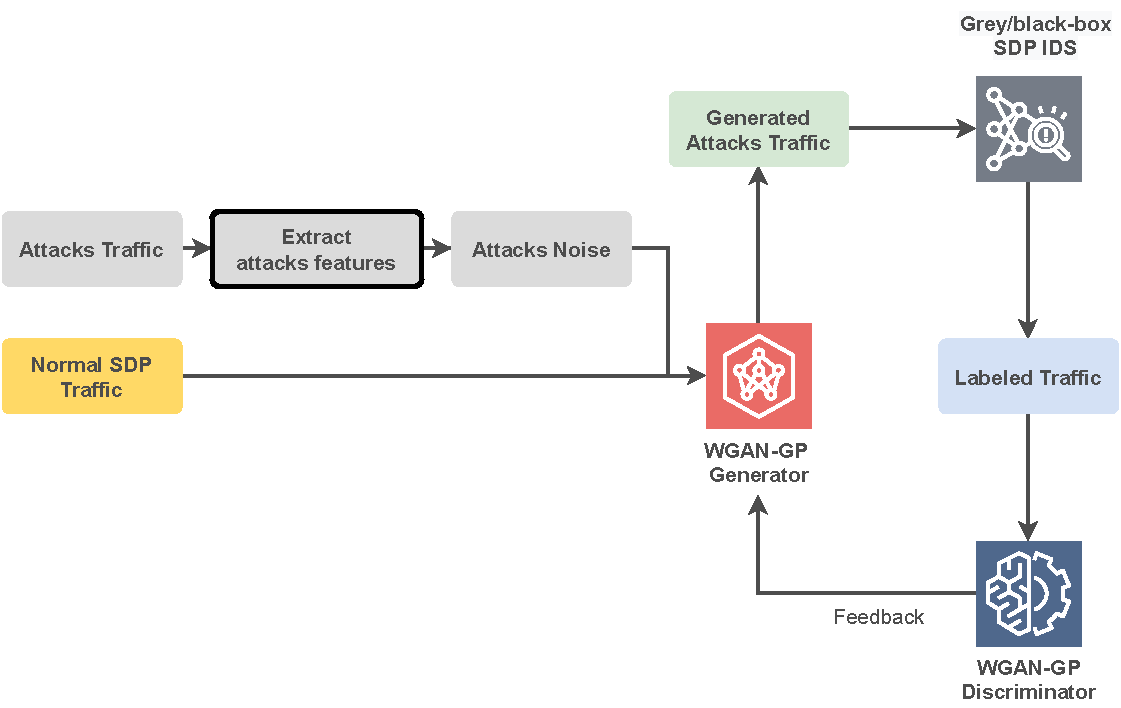
\includegraphics[width=.7\textwidth]{Figures/Harpe-WGAN-GP}
    \caption{\label{fig:harpe-architecture} \textit{Harpe} architecture.}
\end{figure*}

This research project proposes a new framework for generating malicious network traffic in
\textit{Software-Defined Perimeter (SDP)} based networks called \textit{Harpe}.
\textit{Harpe's} goal is to demonstrate that, although \textit{SDP}-based networks are much more secure than traditional
networks, they are not invulnerable and, further research is needed on how to improve them.
To demonstrate this, \textit{Harpe} generates malicious traffic that looks enough like normal traffic to fool the
\textit{Intrusion Detection System (IDS)} located in the \textit{SDP Controller}.
This \textit{IDS} is responsible for filtering traffic directed to the \textit{SDP Controller} (the only accessible
element of the architecture) and allowing only authorization and authentication requests, blocking possible attacks
such as denials of service, among others.

Generating malicious traffic that can fool an \textit{SDP's IDS} is not a simple task.
Creating network traffic that closely resembles normal traffic to evade detection can be difficult, as the limited
types of requests that are allowed make it challenging to create variations without being detected.
Furthermore, generating malicious traffic requires specific characteristics that are associated with successful
attacks.
These characteristics are not always easy to identify, as they can vary depending on the type of attack and the
\textit{IDS} being targeted.

\subsection{Harpe architecture}\label{subsec:traffic-generation}

The architecture of \textit{Harpe} is depicted in Figure~\ref{fig:harpe-architecture}.
In this architecture, The \textit{W-GAN} with Gradient Penalty is composed of two key elements: the
\textit{Traffic Generator} and the \textit{Discriminator}.

In order to generate malicious traffic data, the \textit{Harpe} framework requires access to two types of datasets: one
containing benign or normal \textit{SDP} traffic samples and another containing samples of known attack traffic.
A feature selection process is performed on the attack traffic samples to reserving the functional characteristics of
the traffic by taking into consideration the method in Usama’s study~\cite{usama2019generative}.
To generate adversarial traffic, the \textit{Traffic Generator} utilizes normal traffic as a base, and incorporates
noise derived from chosen features of known attack traffic.
The generated traffic is sent to the \textit{Grey/Black-box} \textit{IDS}, which only provides information on whether
or not the traffic is detected as an attack.
The generated traffic already labeled as benign or attack is passed to the \textit{Discriminator}.
The \textit{Discriminator} is a multi-layer neural network that is trained to distinguish between the normal traffic
and the generated adversarial traffic.
Also, the \textit{Discriminator} is trained to learn and imitate the \textit{IDS}’s decision process based on the
\textit{IDS}’s output.
Finally, the \textit{Discriminator} sends feedback to the \textit{Traffic Generator}, whose gradient is back-propagated
from the \textit{Discriminator} to improve the quality of the generated traffic.

\subsubsection{Feature selection}
In order to generate attacks on \textit{IDS} in network environments we have used the \textit{CIC-IDS2017},
\textit{CSE-CIC-IDS2018}, \textit{CIC-DDoS2019}, and \textit{UNSW-NB15} \textit{IDS} datasets.
These datasets contain benign and the most up-to-date common attacks, which resemble the true real-world data
(as \textit{PCAPs} files).
To generate the CSV files with which the framework works, we have used the
\textit{CICFlowmeter-V4.0}~\cite{lashkari2017cicflowmeter} tool from the Canadian Institute For Cybersecurity.
The \textit{CICFlowmeter-V4.0} is a tool that extracts features from \textit{PCAP} files and generates CSV files
as output.

After acquiring the necessary data, the next step is to identify the characteristics of the attacks that we want to
maintain during the generation of adversarial traffic.
The process of extracting features from traffic records for \textit{IDSs} is thoroughly discussed
by Lee et al~\cite{lee2000framework}.
The authors of this work have developed a four-layer feature extraction scheme that is based on the nature of the
attack found in network traffic flows.
These four steps of feature extraction are \textit{Intrinsic} features, \textit{Time-based} features,
\textit{Host-based} features, and \textit{Content-based} features.

The first step in the feature extraction process involves identifying \textit{intrinsic} features of the network
traffic flow.
These features are essential for determining the validity of the traffic and any alteration in these features will
render the traffic invalid.
The second step in the feature extraction process involves extracting \textit{time-based} features.
Any changes to the \textit{time-based} features of network traffic flow will invalidate the network traffic
characteristics.
Then, the \textit{host-based} traffic features were extracted and, in combination with \textit{intrinsic} and
\textit{time-based} features, are necessary for detecting \textit{slow-probe} attacks.
Any changes to these features will not only alter the \textit{host-based} information, but also invalidate the traffic
flow.
Finally, the content-based features are not required for denial of service attacks.
Any alteration in these features will not invalidate the attack.
In this framework, have used the content-based features to generate adversarial traffic.

\subsubsection{Data Generation}

\begin{equation}
    \label{eq:generatorloss}
    Gen_{Loss} = \mathbb{E}_{M \in normalData,N}Dis(M, N_{attacks})))
\end{equation}

The \textit{Traffic Generator} is a neural network with five linear layers, each with a \textit{ReLU} activation
function.
\textit{ReLU} is a rectified linear unit activation function that is used to add non-linearity to the
network ($ReLU(x) = \max(0, x)$).
The generator loss is calculated based on the \textit{Discriminator}’s output, which reflects the similarity between
the generated adversarial traffic and the normal traffic (see Equation~\ref{eq:generatorloss}).
The generator training performs updates to the generator’s weights based on the gradient information from the
similarity score.
The final goal is to minimize the generator loss.

\begin{equation}
    \label{eq:discriminatorloss}
    Dis_{Loss} = \mathbb{E}_{s \in P_{normal}}Dis(s) + \mathbb{E}_{s \in P_{attack}}Dis(s)
\end{equation}

The \textit{Discriminator} is a neural network with five linear layers, each with a \textit{LeakyReLU} activation
function ($LeakyReLU(x) = \max(0.01x, x)$).
The discriminator loss is calculated based on the results of the \textit{Grey/Black-box} \textit{IDS}’s output, which
labels the generated adversarial traffic as either benign or attack (see Equation~\ref{eq:discriminatorloss}).
The $P_{normal}$ and $P_{attack}$ are the normal and attack traffic samples predicted by the
\textit{IDS}, respectively.

\begin{table}[]
    \resizebox{0.8\columnwidth}{!}{%
        \begin{tabular}{lll}
            \hline
            \textbf{Operation} & \textbf{Units} & \textbf{Non-linearity} \\ \hline
            \multicolumn{3}{l}{\textbf{Traffic Generator (Gen)}} \\ \hline
            Linear             & $input\_dim$   & ReLU                   \\
            Linear             & $input\_dim//2$  & ReLU                   \\
            Linear             & $input\_dim//2$  & ReLU                   \\
            Linear             & $input\_dim//2$  & ReLU                   \\
            Linear             & $input\_dim//2$  & ReLU                   \\ \hline
            \multicolumn{3}{l}{\textbf{Discriminator (Dis)}} \\ \hline
            Linear             & $input\_dim$     & ReLU                   \\
            Linear             & $input\_dim\ast2$   & ReLU                   \\
            Linear             & $input\_dim\ast2$   & ReLU                   \\
            Linear             & $input\_dim\ast2$   & ReLU                   \\
            Linear             & $input\_dim//2$  & ReLU                   \\ \hline
        \end{tabular}
    }
    \caption{Architecture of the \textit{Traffic Generator} and \textit{Discriminator}.}
    \label{tab:gan_architecture}
\end{table}

\begin{table}[]
    \resizebox{0.7\columnwidth}{!}{%
        \begin{tabular}{ll}
            \multicolumn{2}{l}{\textbf{Hyperparameters}} \\ \hline
            Optimizer & RMSProp \\
            Learning Rate & 0.0001 \\
            Batch Size & 128 \\
            Iterations & 150 \\
            Weight Clipping & 0.01 \\
            Discriminator Iterations & 5 \\ \hline
        \end{tabular}
    }
    \caption{\textit{W-GAN} hyperparameters.}
    \label{tab:gan_hyperparameters}
\end{table}

The \textit{Generator} and \textit{Discriminator} architectures are described in Table~\ref{tab:gan_architecture},
and the \textit{W-GAN} hyperparameters are described in Table~\ref{tab:gan_hyperparameters}.

\subsubsection{Grey/Black-Box IDS}
The \textit{grey/black-box IDS} in our framework represents the \textit{ML-based IDS} used by the
\textit{SDP Controller} to filter incoming requests.
\textit{Harpe} only needs a binary response on the data it generates to label them as detected or undetected attacks.
To simulate this \textit{IDS}, we have used some of the most widely used and best performing classifiers from related
work.

\subsection{Integration with the SDP}\label{subsec:integration-with-the-sdp}

\begin{figure}
    \centering
    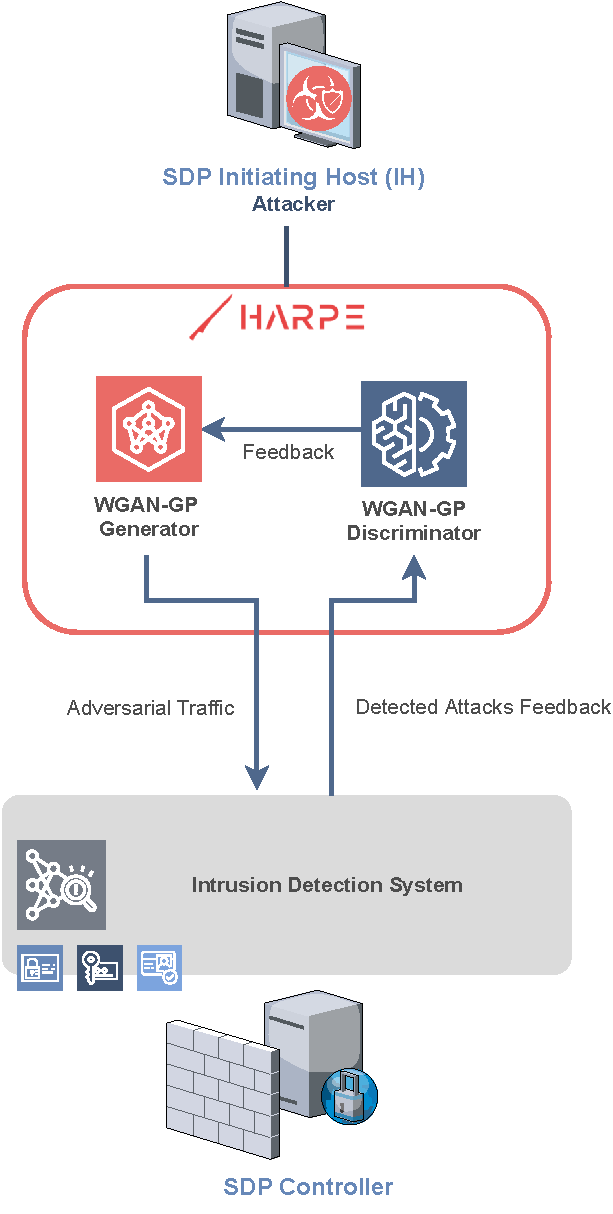
\includegraphics[width=.7\columnwidth]{Figures/Harpe-Integration}
    \caption{\label{fig:harpe-sdp-integration} \textit{Harpe} integration with the \textit{SDP}.}
\end{figure}

The \textit{Harpe} framework is integrated with the \textit{SDP} as shown in Figure~\ref{fig:harpe-sdp-integration}.
The attacker will correspond to the \textit{SDP IH} in the \textit{SDP} network architecture.
The \textit{SDP IH} will generate the adversarial traffic using the \textit{Traffic Generator} and send it to the
\textit{SDP Controller}.
Next, the \textit{IDS} will filter the incoming traffic and \textit{Harpe} will label the samples if they are
detected or undetected attacks.
The \textit{Discriminator} will be trained based on the \textit{IDS}’s output and send the updated weights to the
\textit{Traffic Generator}.
Once we have a trained \textit{Traffic Generator}, we can generate adversarial traffic that is similar to the
normal traffic and is undetected by the \textit{IDS}.

In a typical \textit{SDP} architecture, the \textit{SDP IH} needs to authenticate with the \textit{SDP Controller} to
gain access to the requested resources.
The only type of request in the \textit{SDP} network that can be attacked is the authentication step.
Authenticated requests between an \textit{SDP IH} and an \textit{SDP AH} typically have a short period of validity,
making it difficult for prolonged attacks such as denial of service \textit{(DoS)} to occur.
It should be noted that, in an \textit{SDP} network, there are two types of situations that make it difficult to carry
out attacks on the network.

\begin{itemize}
    \item The network is fully enclosed, where the components are fixed and cannot be altered.
    As a result, no external devices can initiate requests and to launch an attack, one must be part of the network.
    In this case, the locations and values of the \textit{SDP} IHs must be fixed and maintained throughout their
    lifetime in order to be connected to the network.

    \item The \textit{SDP} network allows for some flexibility in the \textit{SDP IH}, with the \textit{SDP Controller}
    being responsible for validation and verification.
    In this case, the \textit{SDP IH} can be moved to a different location, but the \textit{SDP Controller} must
    validate the new location.
    This case is the selected scenario for the \textit{Harpe} framework as it allows more requests types to train the
    \textit{Traffic Generator}.
\end{itemize}


%% ============================================================ V. Evaluation


    \section{Evaluation}\label{sec:evaluation}
    This section introduces the preparation of our experiments to evaluate our proposed framework.
For this purpose, we have deployed an \textit{SDP} network, generated traffic simulating normal behavior to train an
\textit{IDS} model and trained our framework to generate adversarial traffic.

The code that was used and created during the evaluation of our proposal is completely open and accessible.
It can be found on the popular code sharing and collaboration platform,
\textit{GitHub}~\footnote{https://github.com/antonioalfa22/Harpe}.

\subsection{Methodology}\label{subsec:methodology}
To evaluate the performance of our proposed framework, we have designed two environments to test its ability to
generate adversarial traffic that can fool an ML-based \textit{IDS}.

To evaluate the performance of our solution, we first employed \textit{IDS} datasets from previous studies that were
used in traditional network architectures in our test environment.
This approach allows us to assess our solution's ability to generate adversarial traffic that can evade detection by
existing classifiers
Finally, we have developed a second environment to test our solution in an SDP-based network.
The objective of this evaluation environment is to assess the ability of our solution to generate adversarial traffic
that can evade detection by the \textit{IDS} in the \textit{SDP Controller}.
This will provide a comprehensive understanding of the effectiveness of our solution in modern network environments
and its potential to circumvent security mechanisms.

In this study, we have specifically focused on evaluating the performance of our solution against denial of service
\textit{(DoS)} attacks.
This is because \textit{DoS} attacks are a prevalent type of attack and are present in all of the datasets used in our
analysis.
Despite the presence of other types of attacks in these datasets, focusing on \textit{DoS} attacks allows us to have a
specific and consistent benchmark to evaluate our solution's performance.

All the experiments were performed on a \textit{Ubuntu 20.04.5 LTS} machine with an
\textit{Intel(R) Core(TM) i7-7700 CPU @ 3.60GHz} processor and 16 GB of RAM memory.

\subsubsection{Evaluation Metrics}
In order to thoroughly assess the effectiveness of our proposal, we have selected two metrics that were utilized in a
previous study, called \textit{IDSGAN}~\cite{lin2022idsgan}.
These metrics are known as the \textit{Detection Rate (DR)}(described in equation~~\ref{eq:detection_rate}) and the
\textit{Evasion Increase Rate (EIR)} (described in equation~\ref{eq:evasion_increase_rate}).
By utilizing these metrics, we are able to evaluate the performance of \textit{Harpe}, both directly and comparatively.
This allows us to gain a comprehensive understanding of how well our proposal performs in comparison to other similar
methods, and how well it performs overall.
By using these metrics, we can ensure that our proposal is evaluated in a rigorous and objective manner, which will
help us identify areas for improvement and make necessary adjustments for optimal performance.

\begin{equation}
    \label{eq:detection_rate}
    DR = \frac{Attacks TP}{Attacks TP + Attacks FN}
\end{equation}

\begin{equation}
    \label{eq:evasion_increase_rate}
    EIR = 1 - \frac{Adversarial Detection Rate}{Normal Detection Rate}
\end{equation}

\subsubsection{Traditional IDS Environment}
In the traditional environment test scenario, we utilized the \textit{CIC-IDS2017}, \textit{CSE-CIC-IDS2018},
\textit{CIC-DDoS2019}, and \textit{UNSW-NB15} \textit{IDS} datasets to train a set of classifiers.
Our goal is to further train \textit{Harpe} using data from these datasets in order to showcase its capability to
generate adversarial traffic and evaluate its performance against other existing solutions in the field.

The classification algorithms used for the \textit{grey/black-box IDS} are \textit{Support Vector Machines (SVM)},
\textit{Naive Bayes (NB)}, \textit{Multilayer Perceptrons (MLP)}, \textit{Logistic Regression (LR)}, and
\textit{Random Forests (RF)}.

\subsubsection{SDP IDS Environment}
After demonstrating the efficacy of our solution in generating adversarial traffic that can evade detection by
\textit{grey/black-box} \textit{IDSs} in traditional network environments, it is necessary to extend the evaluation of
our solution to its ability to exploit vulnerabilities in \textit{Software-Defined Perimeter (SDP)}-based networks.

In order to evaluate the performance of our solution in a \textit{SDP}-based network architecture, we have designed a
test scenario that simulates the behavior of a \textit{SDP} network using the Waverley Labs implementation.
This test scenario consists of a \textit{SDP} network that is composed of a \textit{SDP Controller}, two
\textit{SDP Initiating Hosts (IHs)}, and one \textit{SDP Accepting Host (AH)}.

We have deployed a traffic generator to generate normal traffic in the \textit{SDP} network.
This traffic generator is responsible for generating traffic that simulates the behavior of a \textit{SDP} network.
Additionally, we have included the \textit{CICFlowmeter-V4.0} tool to generate the \textit{grey/black-box} \textit{IDS}
dataset from the traffic generated.

Finally, we have trained our \textit{grey/black-box} \textit{IDS} with the \textit{Support Vector Machines (SVM)},
\textit{Naive Bayes (NB)}, \textit{Multilayer Perceptrons (MLP)}, \textit{Decision Trees (DT)},
\textit{Logistic Regression (LR)}, and \textit{Random Forests (RF)} classifiers.

\subsection{Results}\label{subsec:results}
Below, we present the results of our experiments in the two evaluation environments.
The functional characteristics used by \textit{DoS} attacks are intrinsic and time-based, namely \textit{Flow Duration,
    Active Mean, Average Packet Size, Packet Length Std, Flow IAT Mean, PSH Flag Count, Idle Max}
~\cite{CSE-CIC-IDS2018, usama2019generative}.

\subsubsection{Traditional IDS Environment}
Prior to the training of the \textit{IDS} models, we performed a common pre-processing step on the data from all
datasets.
This step is crucial as it allows us to standardize the datasets, ensuring that we are working in the same way with
each of them.
To accomplish this, we use a combination of \textit{sklearn} functions such as \textit{StandardScaler} and
\textit{OneHotEncoder}.
The \textit{StandardScaler} function is used to standardize our datasets by removing the mean and scaling to unit
variance.
Meanwhile, the \textit{OneHotEncoder} function is used to convert categorical variables into a format that can be
provided to machine learning algorithms to improve performance.
These tools help us to ensure that our datasets are in a consistent format and ready for training.
In addition to standardizing the datasets, we also perform additional steps to further prepare the data for training
our \textit{IDS} models.
One of these steps is to apply the \textit{log1p} function, which is used to perform $\log(1+x)$ transformation on the
data.
This transformation is applied to help alleviate the presence of outliers and skewed data in our datasets.
Additionally, we also eliminate highly correlated variables.
This is done to remove any redundant information and to prevent multi-collinearity.
This is an important step, as highly correlated variables can lead to instability in our models, thus reducing their
accuracy.
By applying these additional pre-processing steps, we are able to ensure that the data is in the best possible format
for training our \textit{IDS} models.

% ========================================================================== UNSW-NB15

\begin{table}[t]
    \resizebox{\columnwidth}{!}{%
        \begin{tabular}{r|ll|ll|l}
            \cline{2-5}
            \multicolumn{1}{l|}{} & \multicolumn{2}{c|}{\textbf{Accuracy (\%)}} & \multicolumn{2}{c|}{\textbf{Detection Rate (\%)}} &  \\ \cline{2-6}
            \multicolumn{1}{l|}{}              & \multicolumn{1}{c}{\textbf{Origin}} & \multicolumn{1}{c|}{\textbf{Adversarial}} & \multicolumn{1}{c}{\textbf{Origin}} & \multicolumn{1}{c|}{\textbf{Adversarial}} & \multicolumn{1}{c|}{\textbf{EIR}} \\ \hline
            \multicolumn{1}{|r|}{\textbf{MLP}} & 78.16800                            & 45.15392                                  & 87.23630                            & 0.00000                                   & \multicolumn{1}{l|}{1.00000}      \\
            \multicolumn{1}{|r|}{\textbf{SVM}} & 85.52806                            & 40.46552                                  & 82.57736                            & 0.00000                                   & \multicolumn{1}{l|}{1.00000}      \\
            \multicolumn{1}{|r|}{\textbf{NB}}  & 72.22800                            & 39.49882                                  & 75.73822                            & 0.00000                                   & \multicolumn{1}{l|}{1.00000}      \\
            \multicolumn{1}{|r|}{\textbf{LR}}  & 85.47430                            & 40.57214                                  & 82.59692                            & 0.81922                                   & \multicolumn{1}{l|}{0.99014}      \\
            \multicolumn{1}{|r|}{\textbf{RF}}  & 74.81544                            & 42.18392                                  & 80.70917                            & 0.00000                                   & \multicolumn{1}{l|}{1.00000}      \\ \hline
        \end{tabular}
    }
    \caption{Performance of the \textit{IDSs} classifiers with adversarial traffic on the \textit{UNSW-NB15} dataset.
    \label{tab:adversarial-ids-classifiers-unsw-nb15}}
\end{table}

\begin{figure}
    \centering
    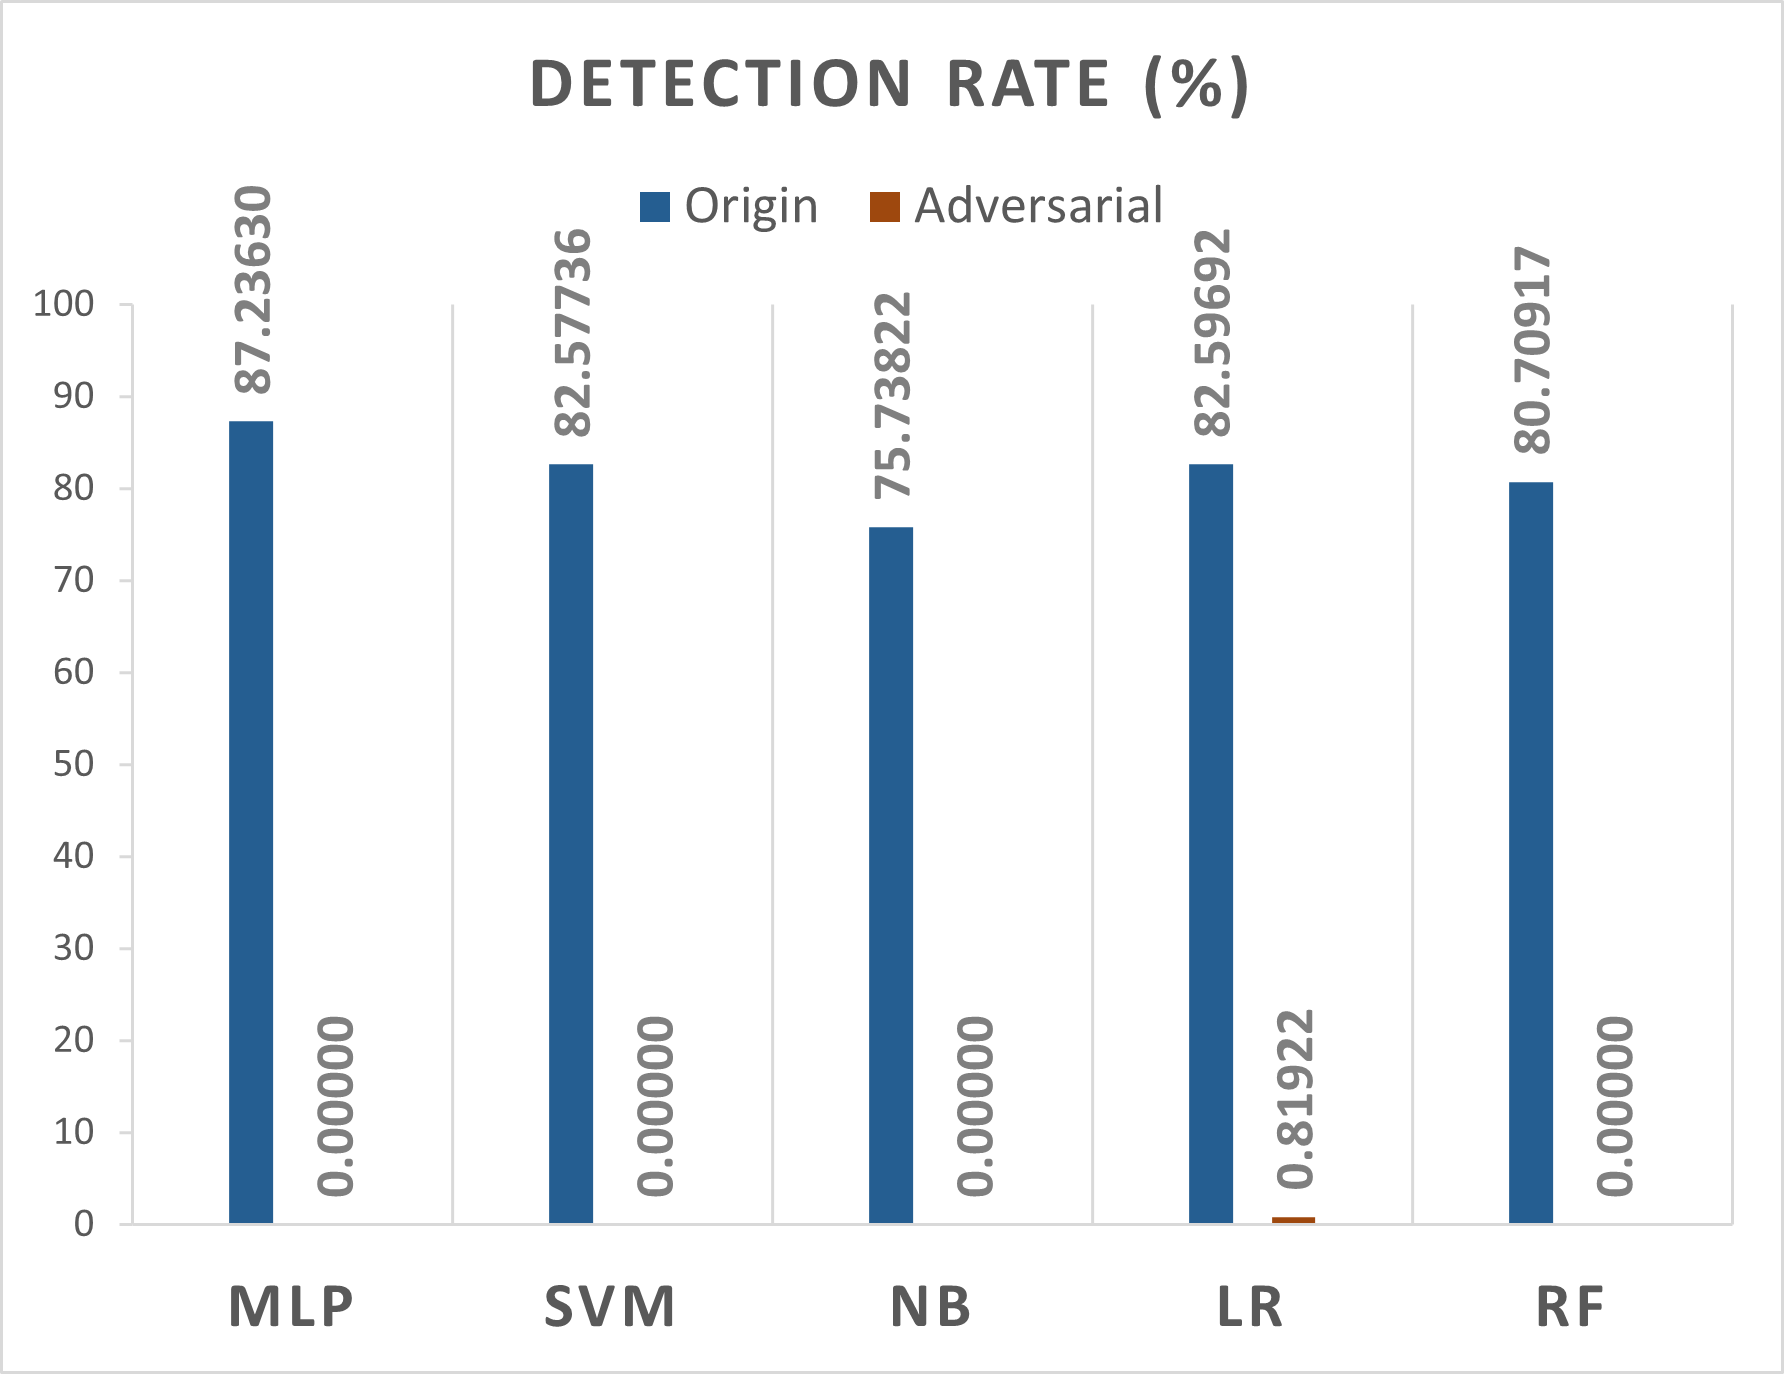
\includegraphics[width=.95\columnwidth]{Figures/UNSW-NB15}
    \caption{\label{fig:unsw-nb15-adversarial} \textit{UNSW-NB15} detection rate.}
\end{figure}

% ========================================================================== CIC-IDS2017
\begin{table}[t]
    \resizebox{\columnwidth}{!}{%
        \begin{tabular}{r|ll|ll|l}
            \cline{2-5}
            \multicolumn{1}{l|}{} & \multicolumn{2}{c|}{\textbf{Accuracy (\%)}} & \multicolumn{2}{c|}{\textbf{Detection Rate (\%)}} &  \\ \cline{2-6}
            \multicolumn{1}{l|}{} & \multicolumn{1}{c}{\textbf{Origin}} & \multicolumn{1}{c|}{\textbf{Adversarial}} & \multicolumn{1}{c}{\textbf{Origin}} & \multicolumn{1}{c|}{\textbf{Adversarial}} & \multicolumn{1}{c|}{\textbf{EIR}} \\ \hline
            \multicolumn{1}{|r|}{\textbf{MLP}} & 89.70249 & 43.17501 & 97.80681 & 0.00000 & \multicolumn{1}{l|}{1.00000} \\
            \multicolumn{1}{|r|}{\textbf{SVM}} & 93.95127 & 48.35813 & 95.48084 & 0.00000 & \multicolumn{1}{l|}{1.00000} \\
            \multicolumn{1}{|r|}{\textbf{NB}} & 97.83296 & 47.85404 & 95.74709 & 0.00000 & \multicolumn{1}{l|}{1.00000} \\
            \multicolumn{1}{|r|}{\textbf{LR}} & 92.30762 & 47.07897 & 93.84646 & 0.00000 & \multicolumn{1}{l|}{1.00000} \\
            \multicolumn{1}{|r|}{\textbf{RF}} & 97.92636 & 54.34136 & 91.54804 & 0.00000 & \multicolumn{1}{l|}{1.00000} \\ \hline
        \end{tabular}
    }
    \caption{Performance of the \textit{IDSs} classifiers with adversarial traffic on the \textit{CIC-IDS2017} dataset.
    \label{tab:adversarial-ids-classifiers-cic-ids-2017}}
\end{table}

\begin{figure}
    \centering
    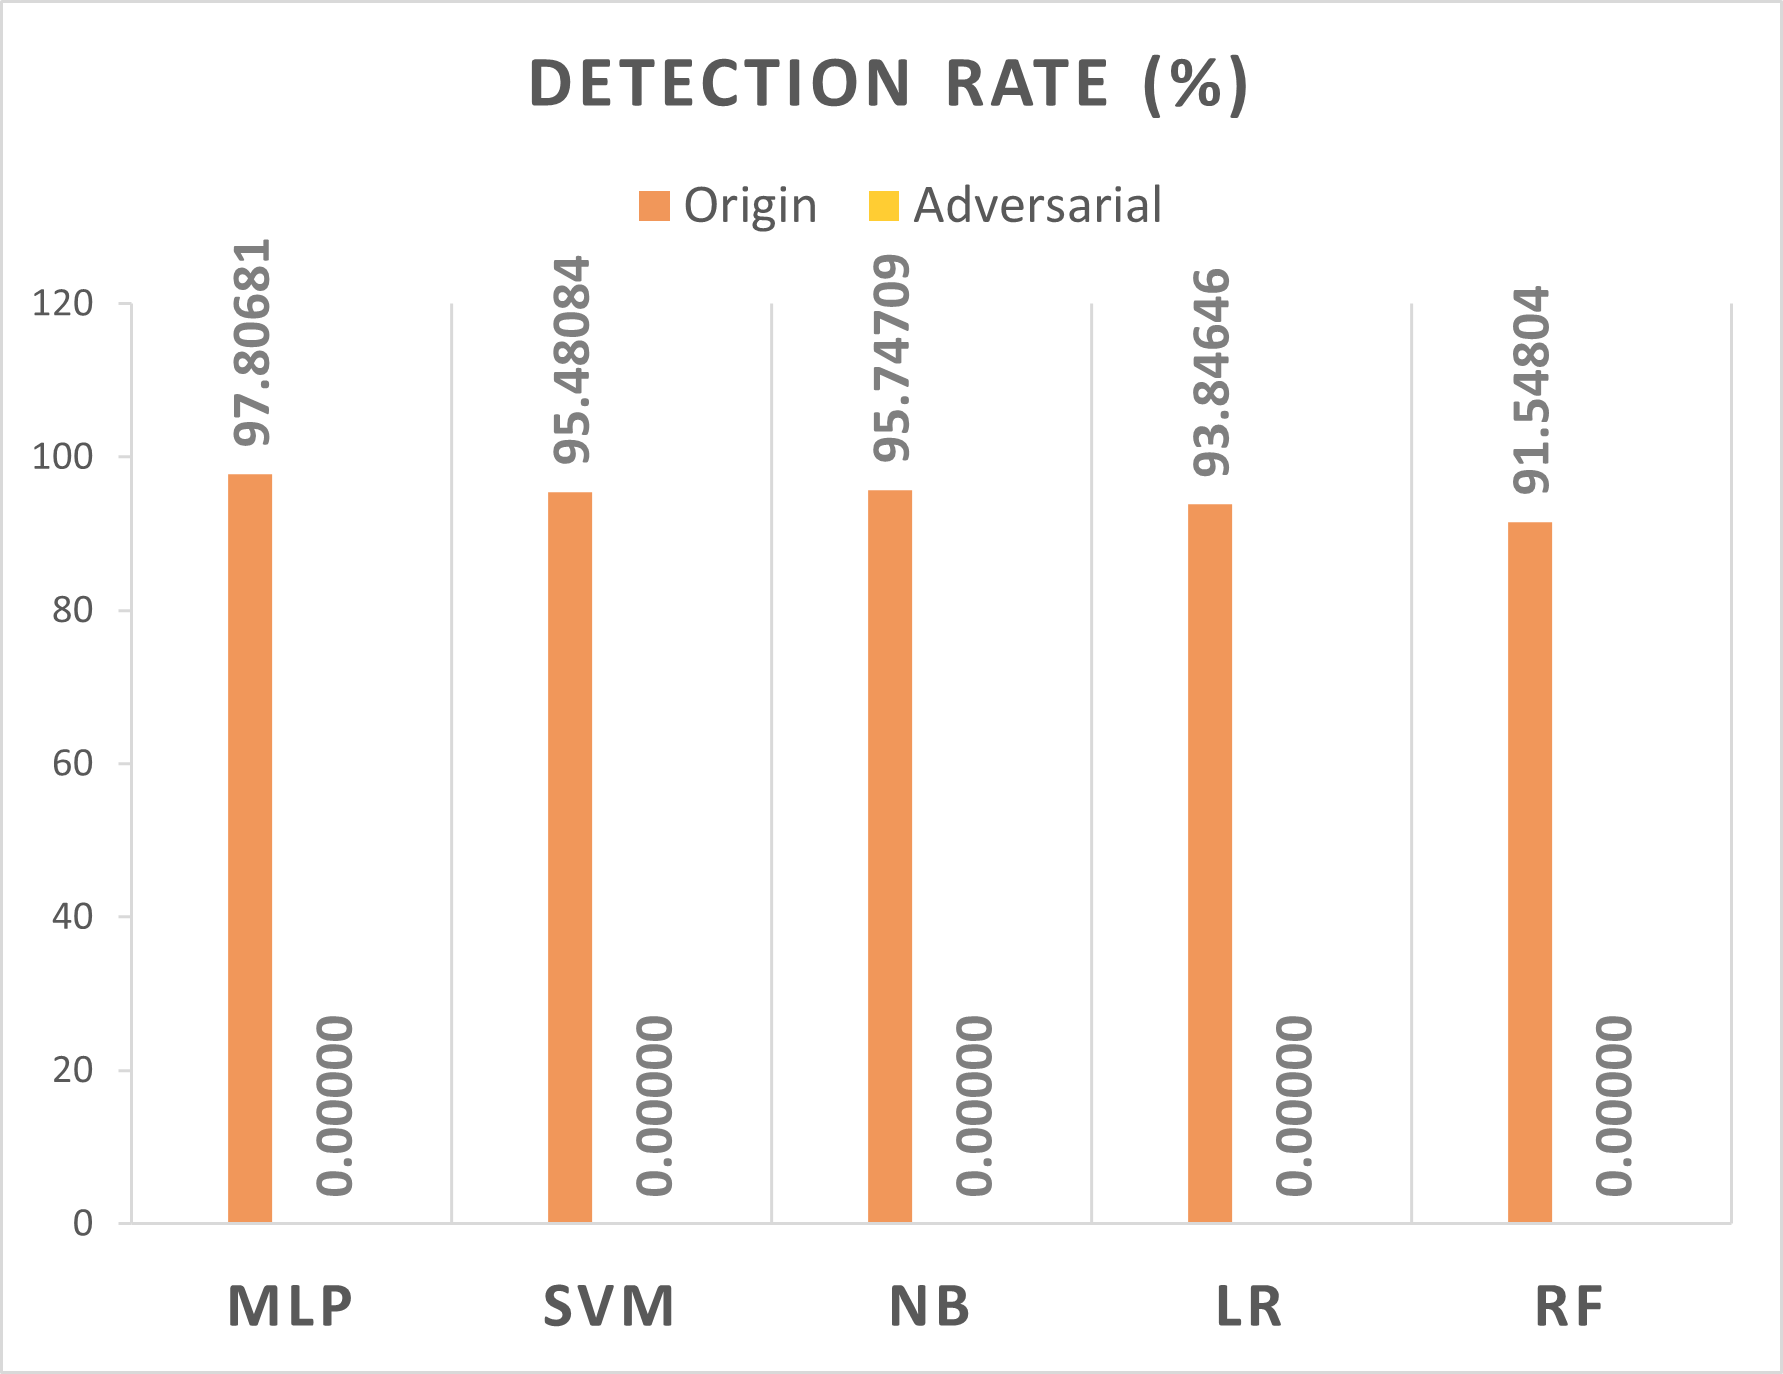
\includegraphics[width=.95\columnwidth]{Figures/CIC-IDS-2017}
    \caption{\label{fig:cic-ids2017-adversarial} \textit{CIC-IDS2017} detection rate.}
\end{figure}

% ========================================================================== CSE-CIC-IDS2018
\begin{table}[t]
    \resizebox{\columnwidth}{!}{%
        \begin{tabular}{r|ll|ll|l}
            \cline{2-5}
            \multicolumn{1}{l|}{} & \multicolumn{2}{c|}{\textbf{Accuracy (\%)}} & \multicolumn{2}{c|}{\textbf{Detection Rate (\%)}} &  \\ \cline{2-6}
            \multicolumn{1}{l|}{} & \multicolumn{1}{c}{\textbf{Origin}} & \multicolumn{1}{c|}{\textbf{Adversarial}} & \multicolumn{1}{c}{\textbf{Origin}} & \multicolumn{1}{c|}{\textbf{Adversarial}} & \multicolumn{1}{c|}{\textbf{EIR}} \\ \hline
            \multicolumn{1}{|r|}{\textbf{MLP}} & 89.03803 & 47.04617 & 94.76926 & 0.03464 & \multicolumn{1}{l|}{0.99963} \\
            \multicolumn{1}{|r|}{\textbf{SVM}} & 95.45637 & 45.35497 & 91.99673 & 0.00000 & \multicolumn{1}{l|}{1.00000} \\
            \multicolumn{1}{|r|}{\textbf{NB}} & 96.72028 & 48.55712 & 92.82482 & 0.00000 & \multicolumn{1}{l|}{1.00000} \\
            \multicolumn{1}{|r|}{\textbf{LR}} & 91.52872 & 44.39624 & 97.91123 & 0.47354 & \multicolumn{1}{l|}{0.99516} \\
            \multicolumn{1}{|r|}{\textbf{RF}} & 98.20424 & 56.16009 & 98.97865 & 0.00000 & \multicolumn{1}{l|}{1.00000} \\ \hline
        \end{tabular}
    }
    \caption{Performance of the \textit{IDSs} classifiers with adversarial traffic on the \textit{CSE-CIC-IDS2018} dataset.
    \label{tab:adversarial-ids-classifiers-cic-ids-2018}}
\end{table}

\begin{figure}
    \centering
    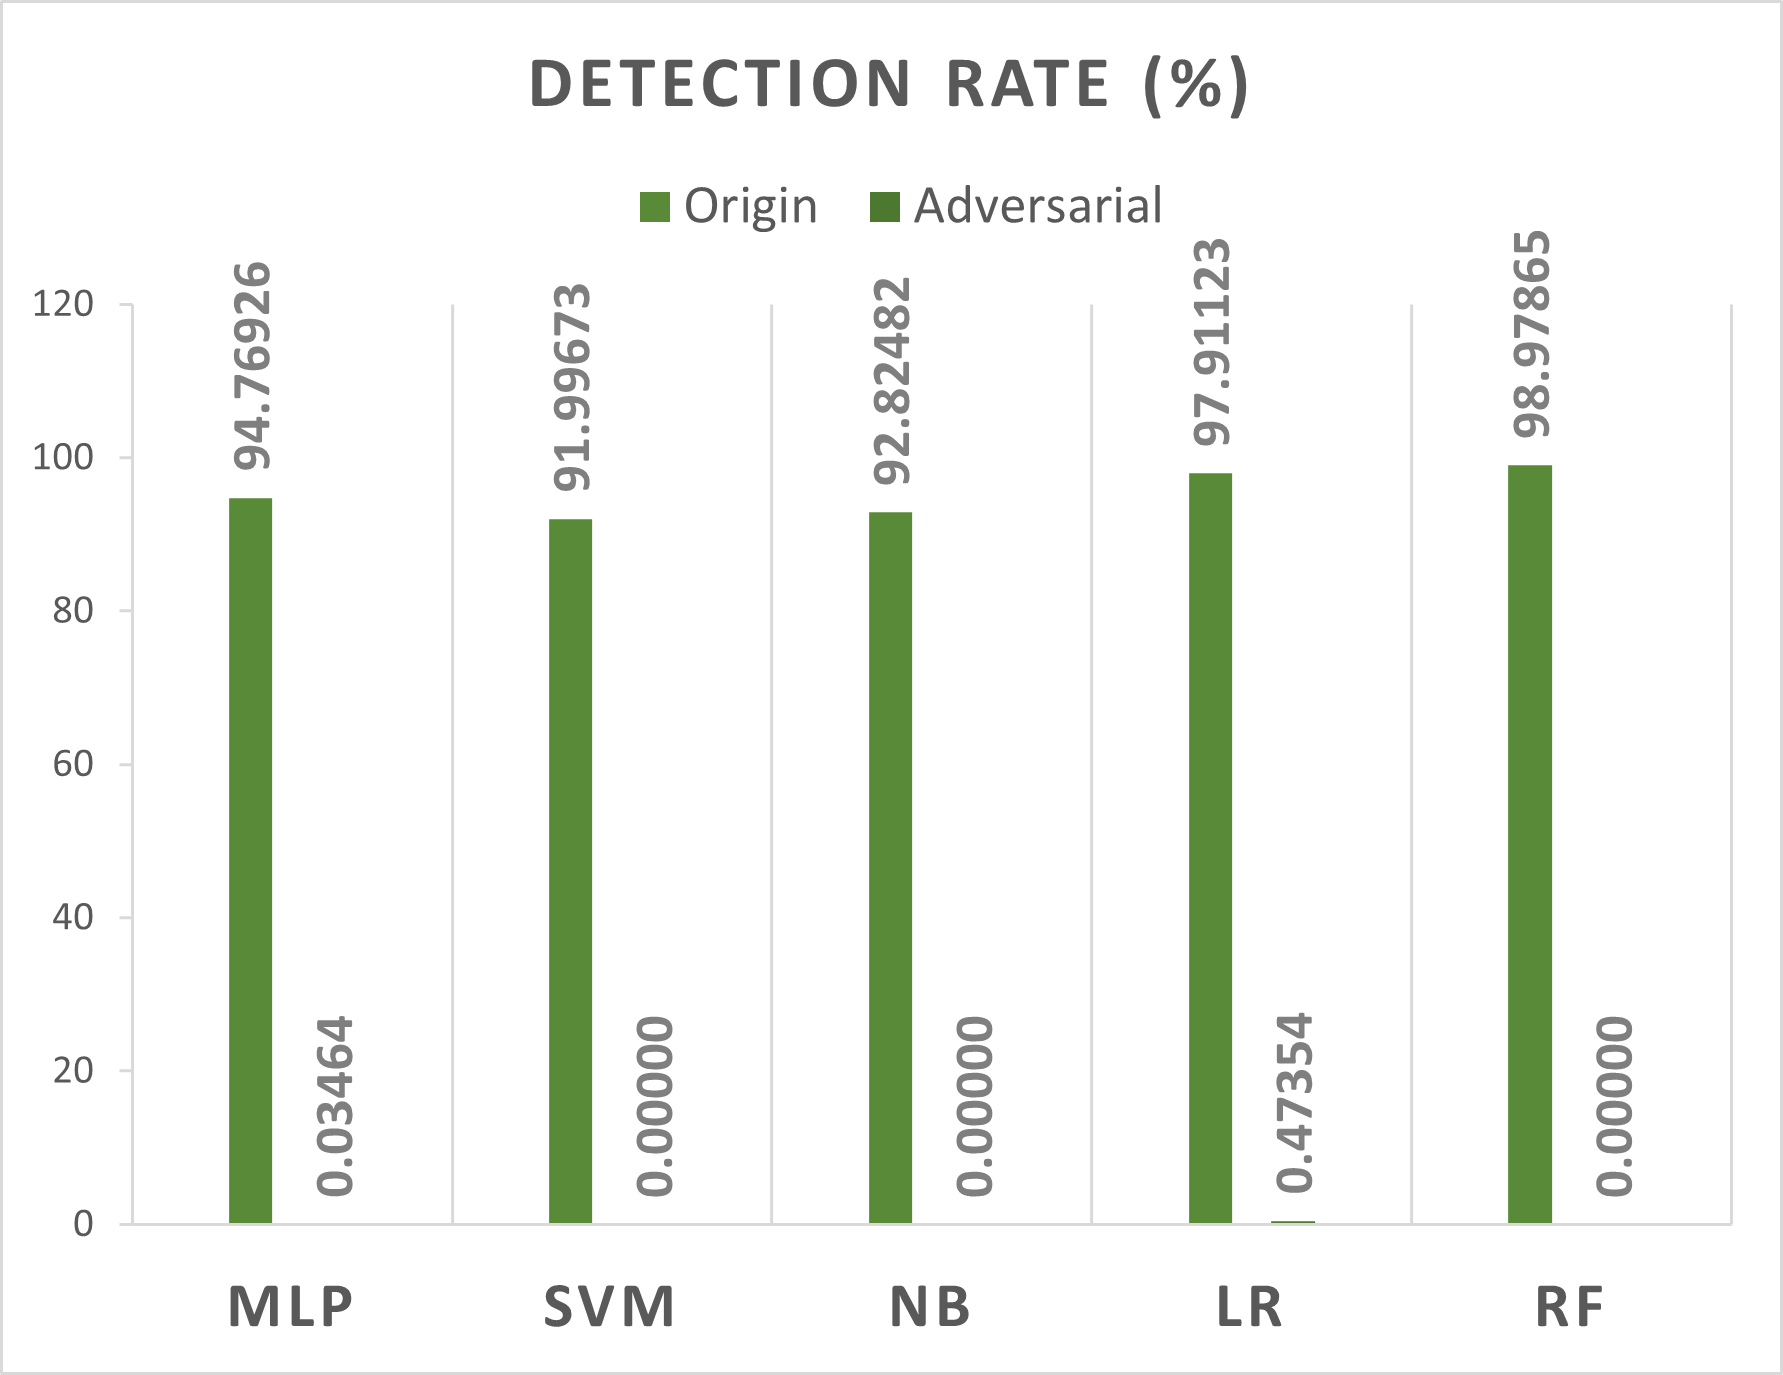
\includegraphics[width=.95\columnwidth]{Figures/CIC-IDS-2018}
    \caption{\label{fig:cic-ids2018-adversarial} \textit{CSE-CIC-IDS2018} detection rate.}
\end{figure}
% ========================================================================== CIC-DDoS2019
\begin{table}[t]
    \resizebox{\columnwidth}{!}{%
        \begin{tabular}{r|ll|ll|l}
            \cline{2-5}
            \multicolumn{1}{l|}{} & \multicolumn{2}{c|}{\textbf{Accuracy (\%)}} & \multicolumn{2}{c|}{\textbf{Detection Rate (\%)}} &  \\ \cline{2-6}
            \multicolumn{1}{l|}{} & \multicolumn{1}{c}{\textbf{Origin}} & \multicolumn{1}{c|}{\textbf{Adversarial}} & \multicolumn{1}{c}{\textbf{Origin}} & \multicolumn{1}{c|}{\textbf{Adversarial}} & \multicolumn{1}{c|}{\textbf{EIR}} \\ \hline
            \multicolumn{1}{|r|}{\textbf{MLP}} & 87.73115 & 48.70946 & 87.06869 & 0.00000 & \multicolumn{1}{l|}{1.00000} \\
            \multicolumn{1}{|r|}{\textbf{SVM}} & 85.45995 & 44.68655 & 84.43590 & 0.00000 & \multicolumn{1}{l|}{1.00000} \\
            \multicolumn{1}{|r|}{\textbf{NB}} & 86.16776 & 47.13445 & 85.14369 & 0.00000 & \multicolumn{1}{l|}{1.00000} \\
            \multicolumn{1}{|r|}{\textbf{LR}} & 83.96291 & 45.23399 & 85.20754 & 0.00000 & \multicolumn{1}{l|}{1.00000} \\
            \multicolumn{1}{|r|}{\textbf{RF}} & 91.42235 & 46.93493 & 84.20779 & 0.00000 & \multicolumn{1}{l|}{1.00000} \\ \hline
        \end{tabular}
    }
    \caption{Performance of the \textit{IDSs} classifiers with adversarial traffic on the \textit{CIC-DDoS2019} dataset.
    \label{tab:adversarial-ids-classifiers-cic-ids-2019}}
\end{table}

\begin{figure}
    \centering
    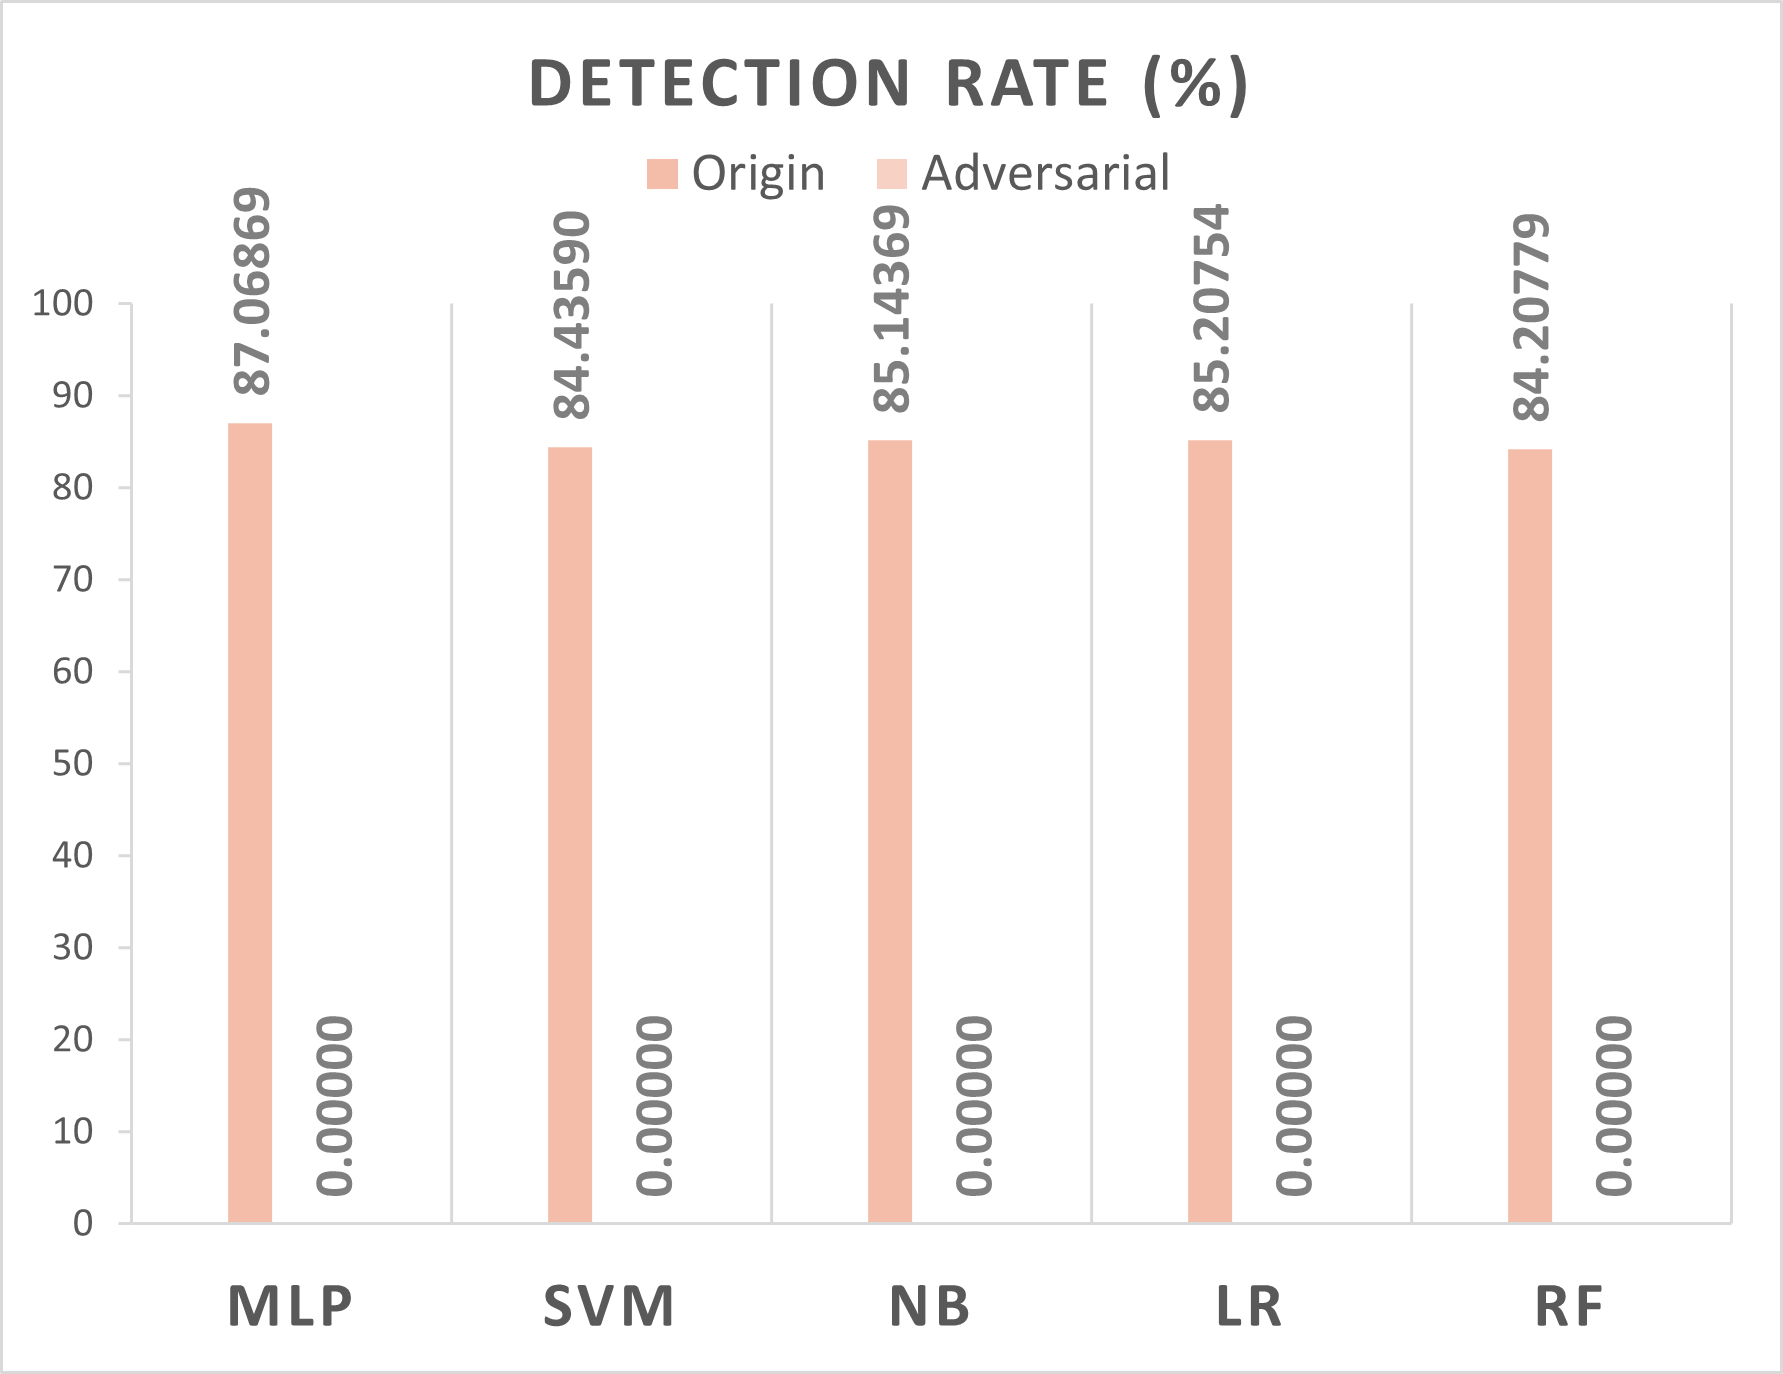
\includegraphics[width=.95\columnwidth]{Figures/CIC-IDS-2019}
    \caption{\label{fig:cic-ids2019-adversarial} \textit{CIC-DDoS2019} detection rate.}
\end{figure}

In this study, we begin our analysis with the \textit{UNSW-NB15} dataset.
The results of this analysis can be observed in Table~\ref{tab:adversarial-ids-classifiers-unsw-nb15} and in the
Figure~\ref{fig:unsw-nb15-adversarial}.
From the table, it is clear to see that the \textit{Detection Rate (DR)} and \textit{Evasion Increase Rate (EIR)}
metrics are quite high.
This indicates that almost all the adversarial traffic generated with our \textit{Harpe} framework is able to fool all
the \textit{IDS} models, and is able to evade detection as an attack.

In the \textit{CIC-IDS2017} (Table~\ref{tab:adversarial-ids-classifiers-cic-ids-2017} and
Figure~\ref{fig:cic-ids2017-adversarial}), \textit{CSE-CIC-IDS2018}
(Table~\ref{tab:adversarial-ids-classifiers-cic-ids-2018} and Figure~\ref{fig:cic-ids2018-adversarial})
and \textit{CIC-DDoS2019} (Table~\ref{tab:adversarial-ids-classifiers-cic-ids-2019} and
Figure~\ref{fig:cic-ids2019-adversarial})
datasets, as in the previous dataset, we can see how by generating adversarial network traffic with the \textit{Harpe}
framework we greatly reduce the \textit{Detection Rate} and obtain values very close to the maximum in the
\textit{Evasion Increase Rate}.
As a consequence, the \textit{accuracy} of the IDS classification algorithms is greatly reduced.

These results indicate that the \textit{Harpe} framework is able to successfully create adversarial attacks on network
traffic that are practically undetectable by the majority of traditional \textit{IDS} systems,
as well as other solutions such as \textit{IDSGAN}, \textit{attackGAN}, and \textit{DIGFuPAS}.
This is a significant achievement as it highlights the framework's ability to bypass the security measures put in place
by these systems.

\subsubsection{SDP IDS Environment}
In order to test our solution in an \textit{SDP-based} network environment, we needed to generate our dataset.
To do this, we developed a tool that simulates traffic in an \textit{SDP network} from two
\textit{SDP Initiating Hosts (IH)} to one \textit{SDP Accepting Host (AH)} using an \textit{Apache} web server.
In an \textit{SDP} network, a connection between an \textit{SDP IH} and an \textit{SDP AH} must be authorized by the
\textit{SDP Controller} prior to any communication taking place.
Because of this, we only stored authentication requests in our dataset, as they are the only type of requests that can
be targeted by attacks.

In general, once a connection is authorized, the \textit{SDP IH} is authorized to access the \textit{SDP AH} for as
long as the \textit{SDP controller} specifies or until the \textit{SDP IH} changes some of its characteristics, such as
IP address, geolocation, etc.
This results in very few authorization requests for the \textit{SDP IH}.
This results in very few authorization requests for a test environment such as the one in this project, where there are
only two \textit{SDP IHs}.
For this reason, we have configured the \textit{SDP Controller} so that the \textit{SDP IH} authorization only lasts
for one request.
This way the \textit{SDP IH} has to make an authorization request for each request it wants to make to the
\textit{SDP AH} web server.

Once we can generate normal or benign traffic, we need to generate attack traffic to train the \textit{grey/black-box}
\textit{IDS}.
To generate this attack traffic, we used the \textit{Slowloris}~\cite{damon2012hands} attack.
\textit{Slowloris} is a type of \textit{DoS} attack that is used to target web servers.
The attack works by consuming all of the available connections on a web server, making it unable to serve legitimate
requests.
This is accomplished by the attacker opening a large number of connections to the web server and keeping them open for
as long as possible.

The generated \textit{SDP}-based network traffic dataset is completely open and can be found in the
\textit{GitHub} repository.
The dataset is composed of two files in \textit{CSV} format, one with the benign traffic and the other with the traffic
generated when executing a \textit{Slowloris DoS} attack.
The dataset has 84 network flow features extracted from the \textit{pcap} files with full packet payloads using the
\textit{CICFlowmeter-V4.0} tool.
The subset with the benign data has 2193 authentication requests made from two \textit{SPD IHs}.
The subset with malicious data has 1203 requests made on one of the \textit{SPD IHs} without prior authentication.

Table~\ref{tab:adversarial-ids-classifiers-sdp} describes the results obtained after training the ML-based \textit{IDS}
for the \textit{SDP-based} network and their \textit{Detection Rates (DR)} for data generated with \textit{Harpe}.
In this scenario, we were only able to achieve detection rates close to 50\% during the training of the \textit{IDS}
classification models.
This may be due to the small amount of data available, as well as to the small variation between them (only two devices
make authentication requests, and one of these devices is the one that subsequently performs the attacks).
However, in real environments and with a larger number of devices, we assume that \textit{IDSs} can achieve much higher
\textit{DR} scores.

\begin{table}[t]
    \resizebox{\columnwidth}{!}{%
        \begin{tabular}{r|ll|ll|l}
            \cline{2-5}
            \multicolumn{1}{l|}{} & \multicolumn{2}{c|}{\textbf{Accuracy (\%)}} & \multicolumn{2}{c|}{\textbf{Detection Rate (\%)}} &  \\ \cline{2-6}
            \multicolumn{1}{l|}{} & \multicolumn{1}{c}{\textbf{Origin}} & \multicolumn{1}{c|}{\textbf{Adversarial}} & \multicolumn{1}{c}{\textbf{Origin}} & \multicolumn{1}{c|}{\textbf{Adversarial}} & \multicolumn{1}{c|}{\textbf{EIR}} \\ \hline
            \multicolumn{1}{|r|}{\textbf{MLP}} & 76.35870 & 49.68038 & 52.71739 & 20.03842 & \multicolumn{1}{l|}{0.61989} \\
            \multicolumn{1}{|r|}{\textbf{SVM}} & 72.75557 & 64.00435 & 37.43255 & 17.10665 & \multicolumn{1}{l|}{0.54300} \\
            \multicolumn{1}{|r|}{\textbf{NB}} & 56.04148 & 55.26820 & 41.92895 & 1.25832 & \multicolumn{1}{l|}{0.96999} \\
            \multicolumn{1}{|r|}{\textbf{LR}} & 68.30679 & 45.23399 & 40.49852 & 8.04726 & \multicolumn{1}{l|}{0.80130} \\
            \multicolumn{1}{|r|}{\textbf{RF}} & 75.28038 & 57.34791 & 55.13747 & 29.51201 & \multicolumn{1}{l|}{0.46476} \\ \hline
        \end{tabular}
    }
    \caption{Performance of the \textit{IDSs} classifiers with adversarial traffic on the generated \textit{SDP}-based network dataset.
    \label{tab:adversarial-ids-classifiers-sdp}}
\end{table}

\begin{figure}
    \centering
    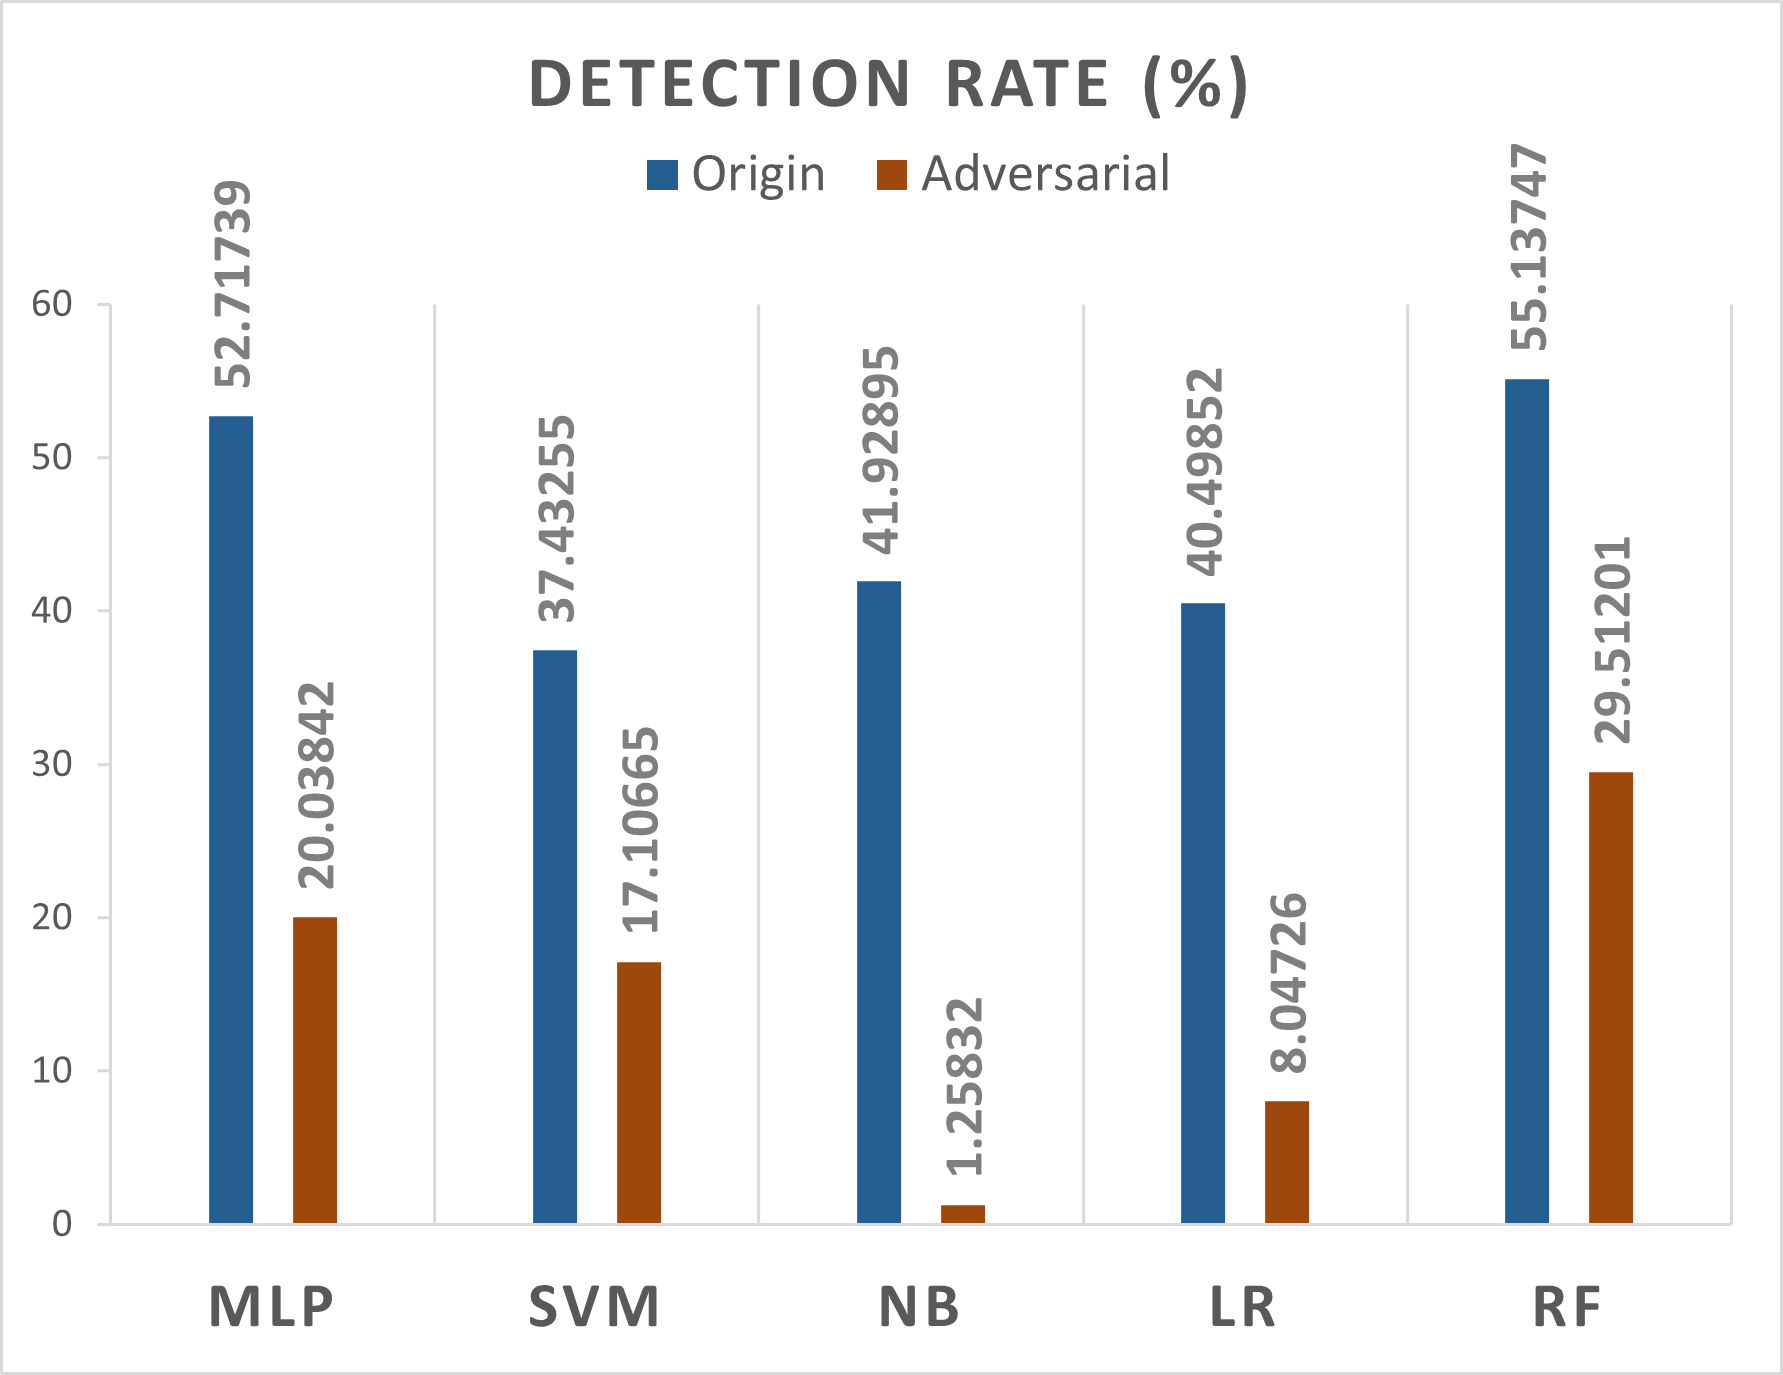
\includegraphics[width=.95\columnwidth]{Figures/SDP-Dataset}
    \caption{\label{fig:dataset-sdp} \textit{SDP}-based network generated dataset detection rate.}
\end{figure}

In this environment, \textit{Harpe} is able to significantly reduce the ability of an \textit{IDS} to distinguish
whether a request is a \textit{DoS} attack or a real authentication request, and performs better against classifiers
using \textit{NB} and \textit{LR}.


%% ============================================================ VI. Conclusions and Future Work


    \section{Conclusions and Future Work}\label{sec:conclusions-and-future-work}
    In conclusion, this paper presents \textit{Apollon}, a new robust defense system against Adversarial Machine Learning attacks
on Intrusion Detection Systems.
\textit{Apollon} utilizes a \textit{Multi-Armed Bandits} model to select the best-suited classifier in
real-time for each input with Thompson sampling, adding a layer of uncertainty to the IDS behavior, that makes it more difficult for
attackers to replicate the IDS and generate adversarial traffic.

Our experimental evaluation on several datasets shows that \textit{Apollon} can successfully detect attacks without compromising
its performance on normal network traffic data, and can prevent attackers from learning the IDS behavior in realistic training times.
These results demonstrate that \textit{Apollon} is an effective defense system against AML attacks in IDS, which
can help to enhance the security of critical systems.
Nevertheless, \textit{Apollon} does not completely eliminate the risk of AML attacks, only mitigates it increasing the
time and effort required by attackers to generate adversarial traffic.

With the aim of improving the performance and robustness of \textit{Apollon}, we plan to explore the use of other \textit{MAB} models and
implementations, such as Bayesian Optimization or Deep Bayesian Bandits.
We also plan to explore the use of other classifiers and ML models, such as requests forecasting models, which can be
used to predict the expected number of requests in the next time window and compare it with the actual number of
requests.
Finally, we plan to explore the use of other datasets, to evaluate the performance of \textit{Apollon} in different network
environments.

%% ============================================================ XI. References

%% Loading bibliography
    \bibliographystyle{ieeetr}
    \bibliography{biblio}



%\vskip3pt

\end{document}